% Created 2011-09-09 Fri 13:16
\documentclass[captions=tableheading]{scrbook}



\subtitle{Second Edition}

\usepackage{lmodern}
\renewcommand{\sfdefault}{lmss}
\renewcommand{\ttdefault}{lmtt}

% needed packages
\usepackage{amsmath}
\usepackage{amssymb}
\usepackage{amsthm}
\usepackage[english]{babel}
\usepackage{epsfig}
\usepackage{fancyvrb}
\usepackage{fixltx2e}
\usepackage{float}
%\usepackage{floatflt}
\usepackage[T1]{fontenc}
\usepackage{footnote}
%\usepackage{graphics}
\usepackage{graphicx}
\usepackage[utf8]{inputenc}
\usepackage{latexsym}
\usepackage{longtable}
\usepackage{makeidx}
\usepackage{marvosym}
\usepackage{multicol}
%\usepackage{pslatex}
%\usepackage{showidx}
\usepackage{soul}
\usepackage{srcltx}
\usepackage{stmaryrd}
\usepackage{subfig}
\usepackage{textcomp}
%\usepackage{theorem}
\usepackage[subfigure]{tocloft}
\usepackage{txfonts}
\usepackage{upgreek}
\usepackage{url}
\usepackage{varioref}
\usepackage{verbatim}
%\usepackage{wasysym}
\usepackage{wrapfig}


% Page setup
\usepackage[paperwidth=7.44in,paperheight=9.69in]{geometry}
\geometry{verbose,tmargin=1in,bmargin=1in,lmargin=1in,rmargin=1in}
\pagestyle{headings}
\setcounter{secnumdepth}{2}
\setcounter{tocdepth}{1}

\makeindex

% PDF settings
\usepackage[hyperref,x11names]{xcolor}
\usepackage[	unicode=true, 
		bookmarks=true, 
		bookmarksnumbered=true, 
		bookmarksopen=true, 
		bookmarksopenlevel=0, 
		breaklinks=true,
		pdfborder={0 0 0},
		backref=page,
		colorlinks=true]{hyperref}
\hypersetup{pdftitle={Introduction to Probability and Statistics Using R},
 		pdfauthor={G. Jay Kerns}, 
		linkcolor=Firebrick4, 
		citecolor=black, 
		urlcolor=SteelBlue4}

% Listings setup
\usepackage{color}
\usepackage{listings}
\lstset{basicstyle={\ttfamily},
	language=R,
	breaklines=true,
	breakatwhitespace=true,
	keywordstyle={\ttfamily},
	numberstyle = {\ttfamily},
	morestring=[b]"
}




%%%%%%%%%%%%%%%%%%%%%%%%%%%%%% LyX specific LaTeX commands.
\providecommand{\LyX}{L\kern-.1667em\lower.25em\hbox{Y}\kern-.125emX\@}
\newcommand{\noun}[1]{\textsc{#1}}
%% Because html converters don't know tabularnewline
\providecommand{\tabularnewline}{\\}

% special logos
\providecommand{\IPSUR}
{\textsc{I\kern 0ex\lower-0.3ex\hbox{\small P}\kern -0.5ex\lower0.4ex\hbox{\footnotesize S}\kern -0.25exU}\kern -0.1ex\lower 0.15ex\hbox{\textsf{\large R}}\@}

%  user defined commands
% special operators

\renewcommand{\vec}[1]{\mbox{\boldmath$#1$}}

\makeatletter

%%%%%%%%%%%%%%%%%%%%%%%%%%%%%% Textclass specific LaTeX commands.

\numberwithin{equation}{section}
\numberwithin{figure}{section}

\theoremstyle{plain}
  \newtheorem{thm}{Theorem}[chapter]
  \newtheorem{fact}[thm]{Fact}
  \newtheorem{ax}[thm]{Axiom}
  \newtheorem{prop}[thm]{Proposition}
  \newtheorem{cor}[thm]{Corollary}
  \newtheorem{assumption}[thm]{Assumption}

\theoremstyle{definition}
  \newtheorem{defn}[thm]{Definition}
  \newtheorem{example}[thm]{Example}
  \newtheorem{xca}{Exercise}[chapter]

\theoremstyle{remark}
  \newtheorem{note}[thm]{Note}
  \newtheorem{rem}[thm]{Remark}
  \newtheorem*{note*}{Note}

\setlength{\cftfignumwidth}{1.5cm}

\@ifundefined{showcaptionsetup}{}{%
 \PassOptionsToPackage{caption=false}{subfig}}
\usepackage{subfig}
\AtBeginDocument{
  \def\labelitemii{\(\circ\)}
}

\makeatother


\newenvironment{exampletoo}{\begin{example}}{\end{example}}


\providecommand{\alert}[1]{\textbf{#1}}

\title{Data Description}
\author{G. Jay Kerns}
\date{\today}

\begin{document}

\maketitle

% Org-mode is exporting headings to 3 levels.

\chapter{Data Description}
\label{sec-1}

\label{cha:Describing-Data-Distributions}


\noindent In this chapter we introduce the different types of data that a statistician is likely to encounter, and in each subsection we give some examples of how to display the data of that particular type. Once we see how to display data distributions, we next introduce the basic properties of data distributions. We qualitatively explore several data sets. Once that we have intuitive properties of data sets, we next discuss how we may numerically measure and describe those properties with descriptive statistics.

\paragraph*{What do I want them to know?}

\begin{itemize}
\item different data types, such as quantitative versus qualitative, nominal versus ordinal, and discrete versus continuous
\item basic graphical displays for assorted data types, and some of their (dis)advantages
\item fundamental properties of data distributions, including center, spread, shape, and crazy observations
\item methods to describe data (visually/numerically) with respect to the properties, and how the methods differ depending on the data type
\item all of the above in the context of grouped data, and in particular, the concept of a factor
\end{itemize}
\section{Types of Data}
\label{sec-1-1}

\label{sec:Types-of-Data}

Loosely speaking, a datum is any piece of collected information, and a data set is a collection of data related to each other in some way. We will categorize data into five types and describe each in turn:

\begin{description}
\item[Quantitative] data associated with a measurement of some quantity on an observational unit,
\item[Qualitative] data associated with some quality or property of an observational unit,
\item[Logical] data which represent true or false and play an important role later,
\item[Missing] data which should be there but are not, and
\item[Other types] everything else under the sun.
\end{description}

In each subsection we look at some examples of the type in question and introduce methods to display them.
\subsection{Quantitative data}
\label{sec-1-1-1}

\label{sub:Quantitative-Data}

Quantitative data are any data that measure or are associated with a measurement of the quantity of something. They invariably assume numerical values. Quantitative data can be further subdivided into two categories. 

\begin{itemize}
\item \emph{Discrete data} take values in a finite or countably infinite set of numbers, that is, all possible values could (at least in principle) be written down in an ordered list. Examples include: counts, number of arrivals, or number of successes. They are often represented by integers, say, 0, 1, 2, \emph{etc}.
\item \emph{Continuous data} take values in an interval of numbers. These are also known as scale data, interval data, or measurement data. Examples include: height, weight, length, time, \emph{etc}. Continuous data are often characterized by fractions or decimals: 3.82, 7.0001, 4 \(\frac{5}{8}\), \emph{etc}.
\end{itemize}

Note that the distinction between discrete and continuous data is not always clear-cut. Sometimes it is convenient to treat data as if they were continuous, even though strictly speaking they are not continuous. See the examples.

\begin{example}
\textbf{Annual Precipitation in US Cities.} The vector \texttt{precip}\index{Data sets!precip@\texttt{precip}} contains average amount of rainfall (in inches) for each of 70 cities in the United States and Puerto Rico. Let us take a look at the data:


\begin{verbatim}
str(precip)
\end{verbatim}

\begin{verbatim}
  Named num [1:70] 67 54.7 7 48.5 14 17.2 20.7 13 43.4 40.2 ...
  - attr(*, "names")= chr [1:70] "Mobile" "Juneau" "Phoenix" "Little Rock" ...
\end{verbatim}


\begin{verbatim}
precip[1:4]
\end{verbatim}

\begin{verbatim}
      Mobile      Juneau     Phoenix Little Rock 
        67.0        54.7         7.0        48.5
\end{verbatim}

The output shows that \texttt{precip} is a numeric vector which has been \emph{named}, that is, each value has a name associated with it (which can be set with the \texttt{names}\index{names@\texttt{names}} function). These are quantitative continuous data.

\end{example}

\begin{example}
\textbf{Lengths of Major North American Rivers.} The U.S. Geological Survey recorded the lengths (in miles) of several rivers in North America. They are stored in the vector \texttt{rivers}\index{Data sets!rivers@\texttt{rivers}} in the \texttt{datasets} package (which ships with base \textsf{R}). See \texttt{?rivers}. Let us take a look at the data with the \texttt{str}\index{str@\texttt{str}} function.


\begin{verbatim}
str(rivers)
\end{verbatim}

\begin{verbatim}
  num [1:141] 735 320 325 392 524 ...
\end{verbatim}


The output says that \texttt{rivers} is a numeric vector of length 141, and the first few values are 735, 320, 325, \emph{etc}. These data are definitely quantitative and it appears that the measurements have been rounded to the nearest mile. Thus, strictly speaking, these are discrete data. But we will find it convenient later to take data like these to be continuous for some of our statistical procedures. 
\end{example}

\begin{example}
\textbf{Yearly Numbers of Important Discoveries.} The vector \texttt{discoveries}\index{Data sets!discoveries@\texttt{discoveries}} contains numbers of “great” inventions/discoveries in each year from 1860 to 1959, as reported by the 1975 World Almanac. Let us take a look at the data:


\begin{verbatim}
str(discoveries)
\end{verbatim}

\begin{verbatim}
  Time-Series [1:100] from 1860 to 1959: 5 3 0 2 0 3 2 3 6 1 ...
\end{verbatim}

\end{example}

The output is telling us that \texttt{discoveries} is a \emph{time series} (see Section \ref{sub:other-data-types} for more) of length 100. The entries are integers, and since they represent counts this is a good example of discrete quantitative data. We will take a closer look in the following sections.
\subsection{Displaying Quantitative Data}
\label{sec-1-1-2}

\label{sub:Displaying-Quantitative-Data}

One of the first things to do when confronted by quantitative data (or any data, for that matter) is to make some sort of visual display to gain some insight into the data's structure. There are almost as many display types from which to choose as there are data sets to plot. We describe some of the more popular alternatives. 

\paragraph*{Strip charts\index{strip chart} (also known as Dot plots)\index{dot plot| see\{strip chart\}}}
\label{par:Strip-charts}

These can be used for discrete or continuous data, and usually look best when the data set is not too large. Along the horizontal axis is a numerical scale above which the data values are plotted. We can do it in \textsf{R} with a call to the \texttt{stripchart}\index{stripchart@\texttt{stripchart}} function. There are three available methods.

\begin{description}
\item[overplot] plots ties covering each other. This method is good to display only the distinct values assumed by the data set.
\item[jitter] adds some noise to the data in the \(y\) direction in which case the data values are not covered up by ties.
\item[stack] plots repeated values stacked on top of one another. This method is best used for discrete data with a lot of ties; if there are no repeats then this method is identical to overplot.
\end{description}

See Figure \ref{fig:stripcharts}, which was produced by the following code.


\begin{verbatim}
stripchart(precip, xlab="rainfall")
stripchart(rivers, method="jitter", xlab="length")
stripchart(discoveries, method="stack", xlab="number")
\end{verbatim}

The leftmost graph is a strip chart of the \texttt{precip} data. The graph shows tightly clustered values in the middle with some others falling balanced on either side, with perhaps slightly more falling to the left. Later we will call this a symmetric distribution, see Section \ref{sub:Shape}. The middle graph is of the \texttt{rivers} data, a vector of length 141. There are several repeated values in the rivers data, and if we were to use the overplot method we would lose some of them in the display. This plot shows a what we will later call a right-skewed shape with perhaps some extreme values on the far right of the display. The third graph strip charts \texttt{discoveries} data which are literally a textbook example of a right skewed distribution.


\begin{verbatim}
par(mfrow = c(3,1)) # 3 plots: 3 rows, 1 column
stripchart(precip, xlab="rainfall")
stripchart(rivers, method="jitter", xlab="length")
stripchart(discoveries, method="stack", xlab="number", ylim = c(0,3))
par(mfrow = c(1,1)) # back to normal
\end{verbatim}



\begin{figure}[ht!]
    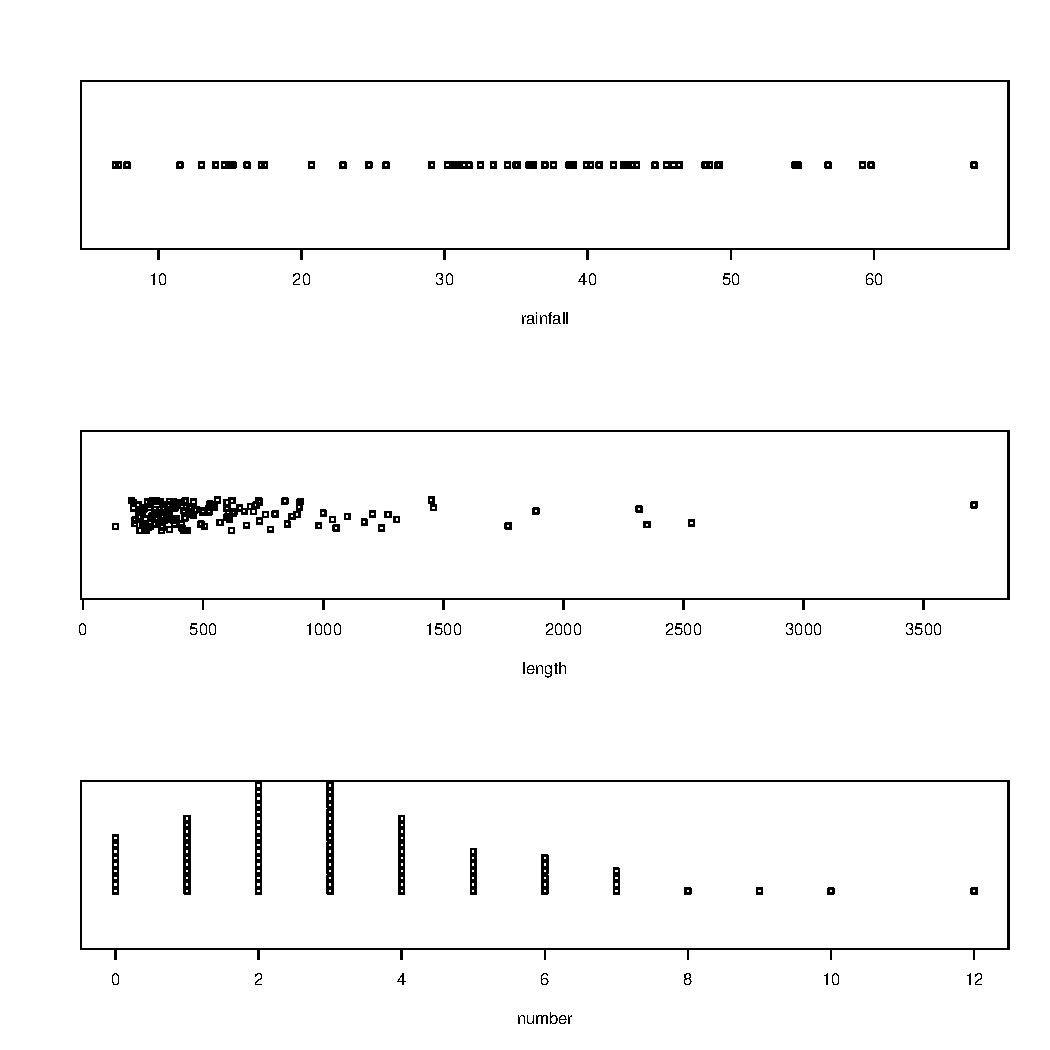
\includegraphics[width=5in, height=4in]{img/stripcharts.pdf}
    \caption[Strip charts of \texttt{precip}, \texttt{rivers}, and \texttt{discoveries}]{\small Three stripcharts of three data sets.  The first graph uses the \texttt{overplot} method, the second the \texttt{jitter} method, and the third the \texttt{stack} method.}
    \label{fig:stripcharts}
  \end{figure}

The \texttt{DOTplot}\index{DOTplot@\texttt{DOTplot}} function in the \texttt{UsingR}\index{R packages!UsingR@\texttt{UsingR}} package \cite{usingr} is another alternative.

\paragraph*{Histogram\index{Histogram}}

These are typically used for continuous data. A histogram is constructed by first deciding on a set of classes, or bins, which partition the real line into a set of boxes into which the data values fall. Then vertical bars are drawn over the bins with height proportional to the number of observations that fell into the bin. 

These are one of the most common summary displays, and they are often misidentified as ``Bar Graphs'' (see below.) The scale on the \(y\) axis can be frequency, percentage, or density (relative frequency). The term histogram was coined by Karl Pearson in 1891, see \cite{Miller}.

\begin{example}
\textbf{Annual Precipitation in US Cities.} We are going to take another look at the \texttt{precip}\index{Data sets!precip@\texttt{precip}} data that we investigated earlier. The strip chart in Figure \ref{fig:Various-stripchart-methods,} suggested a loosely balanced distribution; let us now look to see what a histogram says. 

There are many ways to plot histograms in \textsf{R}, and one of the easiest is with the \texttt{hist}\index{hist@\texttt{hist}} function. The following code produces the plots in Figure \ref{fig:histograms}.


\begin{verbatim}
hist(precip, main = "")
hist(precip, freq = FALSE, main = "")
\end{verbatim}

Notice the argument \texttt{main = ""} which suppresses the main title from being displayed -- it would have said ``Histogram of \texttt{precip}'' otherwise. The plot on the left is a frequency histogram (the default), and the plot on the right is a relative frequency histogram (\texttt{freq = FALSE}). 


\begin{verbatim}
m <- ggplot(as.data.frame(precip), aes(x = precip))
m + geom_histogram()
m + geom_histogram(binwidth = 5)
\end{verbatim}




\begin{verbatim}
par(mfrow = c(1,2)) # 2 plots: 1 row, 2 columns
hist(precip, main = "")
hist(precip, freq = FALSE, main = "")
par(mfrow = c(1,1)) # back to normal
\end{verbatim}



\begin{figure}[ht!]
    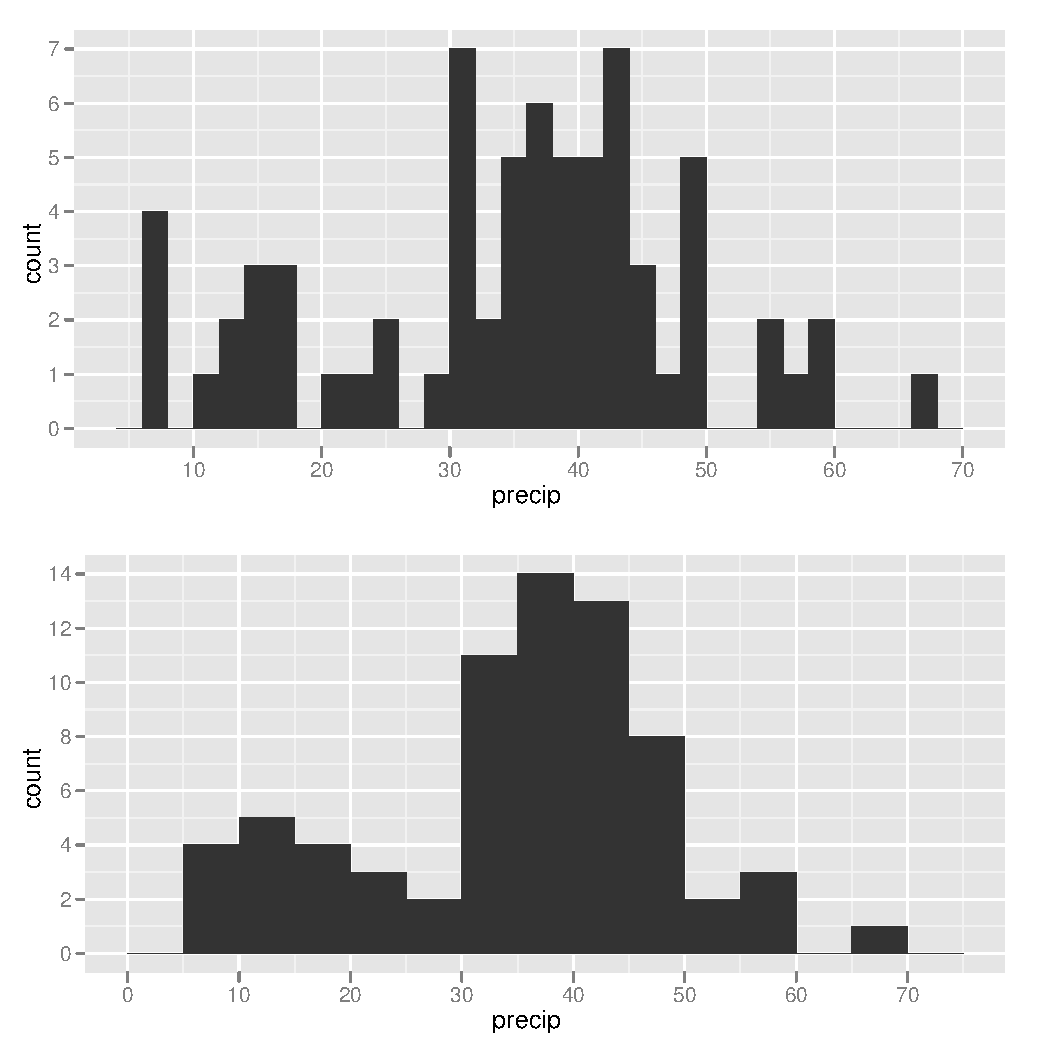
\includegraphics[width=5in, height=4in]{img/histograms.pdf}
    \caption{(Relative) frequency histograms of the \texttt{precip} data}
    \label{fig:histograms}
  \end{figure}

\end{example}

Please mind the biggest weakness of histograms: the graph obtained strongly depends on the bins chosen. Choose another set of bins, and you will get a different histogram. Moreover, there are not any definitive criteria by which bins should be defined; the best choice for a given data set is the one which illuminates the data set's underlying structure (if any). Luckily for us there are algorithms to automatically choose bins that are likely to display well, and more often than not the default bins do a good job. This is not always the case, however, and a responsible statistician will investigate many bin choices to test the stability of the display.

\begin{example}
Recall that the strip chart in Figure \ref{fig:Various-stripchart-methods} suggested a relatively balanced shape to the \texttt{precip} data distribution. Watch what happens when we change the bins slightly (with the \texttt{breaks} argument to \texttt{hist}). See Figure \ref{fig:histograms-bins} which was produced by the following code.



\begin{verbatim}
hist(precip, breaks = 10, main = "")
hist(precip, breaks = 200, main = "")
\end{verbatim}





\begin{figure}[ht!]
    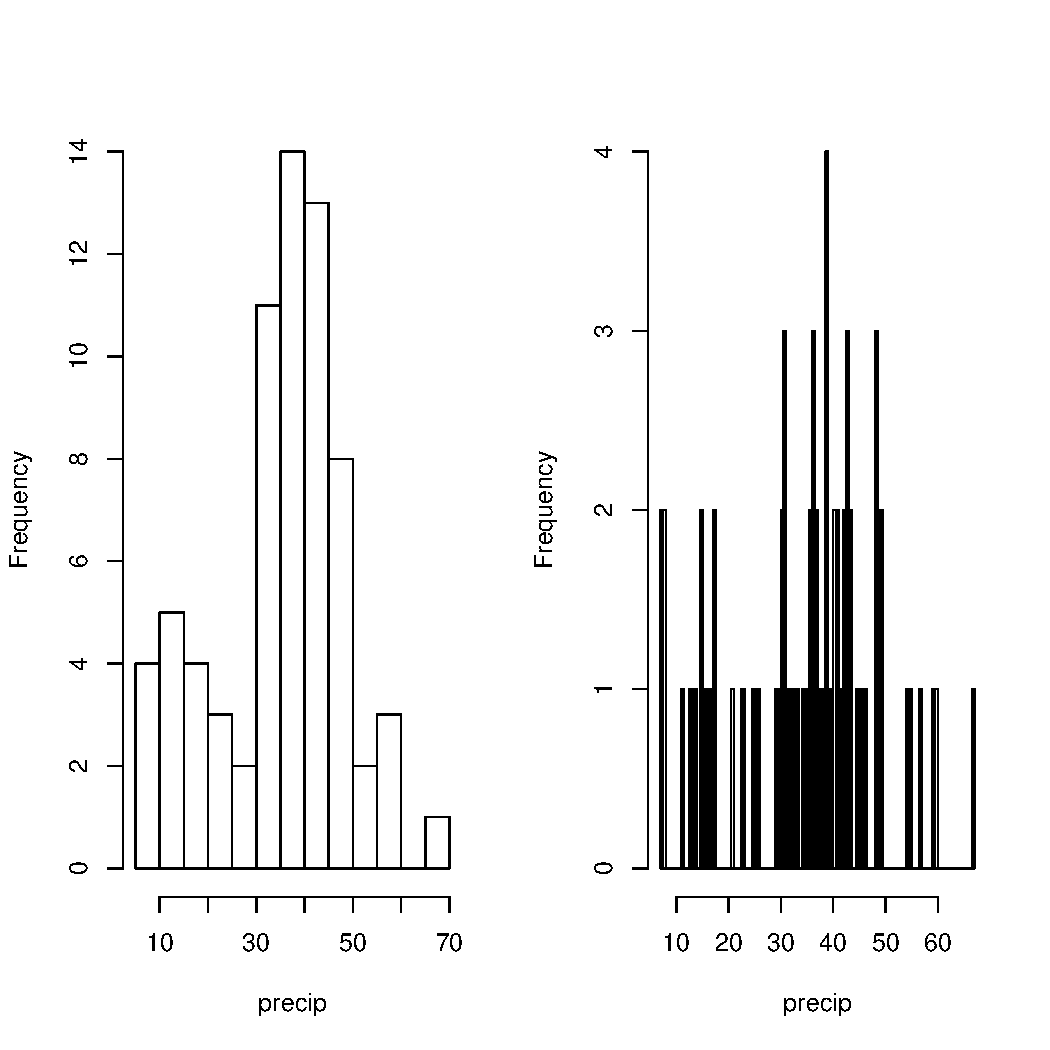
\includegraphics[width=5in, height=4in]{img/histograms-bins.pdf}
    \caption{More histograms of the \texttt{precip} data}
    \label{fig:histograms-bins}
  \end{figure}

The leftmost graph (with \texttt{breaks = 10}) shows that the distribution is not balanced at all. There are two humps: a big one in the middle and a smaller one to the left. Graphs like this often indicate some underlying group structure to the data; we could now investigate whether the cities for which rainfall was measured were similar in some way, with respect to geographic region, for example.

The rightmost graph in Figure \ref{fig:histograms-bins} shows what happens when the number of bins is too large: the histogram is too grainy and hides the rounded appearance of the earlier histograms. If we were to continue increasing the number of bins we would eventually get all observed bins to have exactly one element, which is nothing more than a glorified strip chart.

\end{example}

\paragraph*{Stemplots (more to be said in Section \ref{sec:Exploratory-Data-Analysis})}

Stemplots have two basic parts: \emph{stems} and \emph{leaves}. The final digit of the data values is taken to be a \emph{leaf}, and the leading digit(s) is (are) taken to be \emph{stems}. We draw a vertical line, and to the left of the line we list the stems. To the right of the line, we list the leaves beside their corresponding stem. There will typically be several leaves for each stem, in which case the leaves accumulate to the right. It is sometimes necessary to round the data values, especially for larger data sets.

\begin{example}
\label{exa:-ukdriverdeaths-first}
\texttt{UKDriverDeaths}\index{Data sets!UKDriverDeaths@\texttt{UKDriverDeaths}} is a time series that contains the total car drivers killed or seriously injured in Great Britain monthly from Jan 1969 to Dec 1984. See \texttt{?UKDriverDeaths}. Compulsory seat belt use was introduced on January 31, 1983. We construct a stem and leaf diagram in \textsf{R} with the \texttt{stem.leaf}\index{stem.leaf@\texttt{stem.leaf}} function from the \texttt{aplpack}\index{R packages@\textsf{R} packages!aplpack@\texttt{aplpack}} package\cite{aplpack}.
\end{example}


\begin{verbatim}
library(aplpack)
stem.leaf(UKDriverDeaths, depth = FALSE)
\end{verbatim}


\begin{verbatim}
1 | 2: represents 120
 leaf unit: 10
            n: 192
   10 | 57
   11 | 136678
   12 | 123889
   13 | 0255666888899
   14 | 00001222344444555556667788889
   15 | 0000111112222223444455555566677779
   16 | 01222333444445555555678888889
   17 | 11233344566667799
   18 | 00011235568
   19 | 01234455667799
   20 | 0000113557788899
   21 | 145599
   22 | 013467
   23 | 9
   24 | 7
HI: 2654
\end{verbatim}

The display shows a more or less balanced mound-shaped distribution, with one or maybe two humps, a big one and a smaller one just to its right. Note that the data have been rounded to the tens place so that each datum gets only one leaf to the right of the dividing line.

Notice that the \texttt{depth}s\index{depths} have been suppressed. To learn more about this option and many others, see Section \ref{sec:Exploratory-Data-Analysis}. Unlike a histogram, the original data values may be recovered from the stemplot display -- modulo the rounding -- that is, starting from the top and working down we can read off the data values 1050, 1070, 1110, 1130, and so forth. 

\paragraph*{Index plots}

Done with the \texttt{plot}\index{plot@\texttt{plot}} function. These are good for plotting data which are ordered, for example, when the data are measured over time. That is, the first observation was measured at time 1, the second at time 2, \emph{etc}. It is a two dimensional plot, in which the index (or time) is the \(x\) variable and the measured value is the \(y\) variable. There are several plotting methods for index plots, and we mention two of them:

\begin{description}
\item[spikes] draws a vertical line from the \(x\)-axis to the observation height (\texttt{type = "h"}).
\item[points] plots a simple point at the observation height (=type = ``p''=).
\end{description}


\begin{example}
\textbf{Level of Lake Huron 1875-1972.} Brockwell and Davis \cite{Brockwell1991} give the annual measurements of the level (in feet) of Lake Huron from 1875--1972. The data are stored in the time series \texttt{LakeHuron}\index{Data sets!LakeHuron@\texttt{LakeHuron}}. See \texttt{?LakeHuron}. Figure \ref{fig:indpl-lakehuron} was produced with the following code:


\begin{verbatim}
plot(LakeHuron, type = "h")
plot(LakeHuron, type = "p")
\end{verbatim}

The plots show an overall decreasing trend to the observations, and there appears to be some seasonal variation that increases over time. 





\begin{figure}[ht!]
    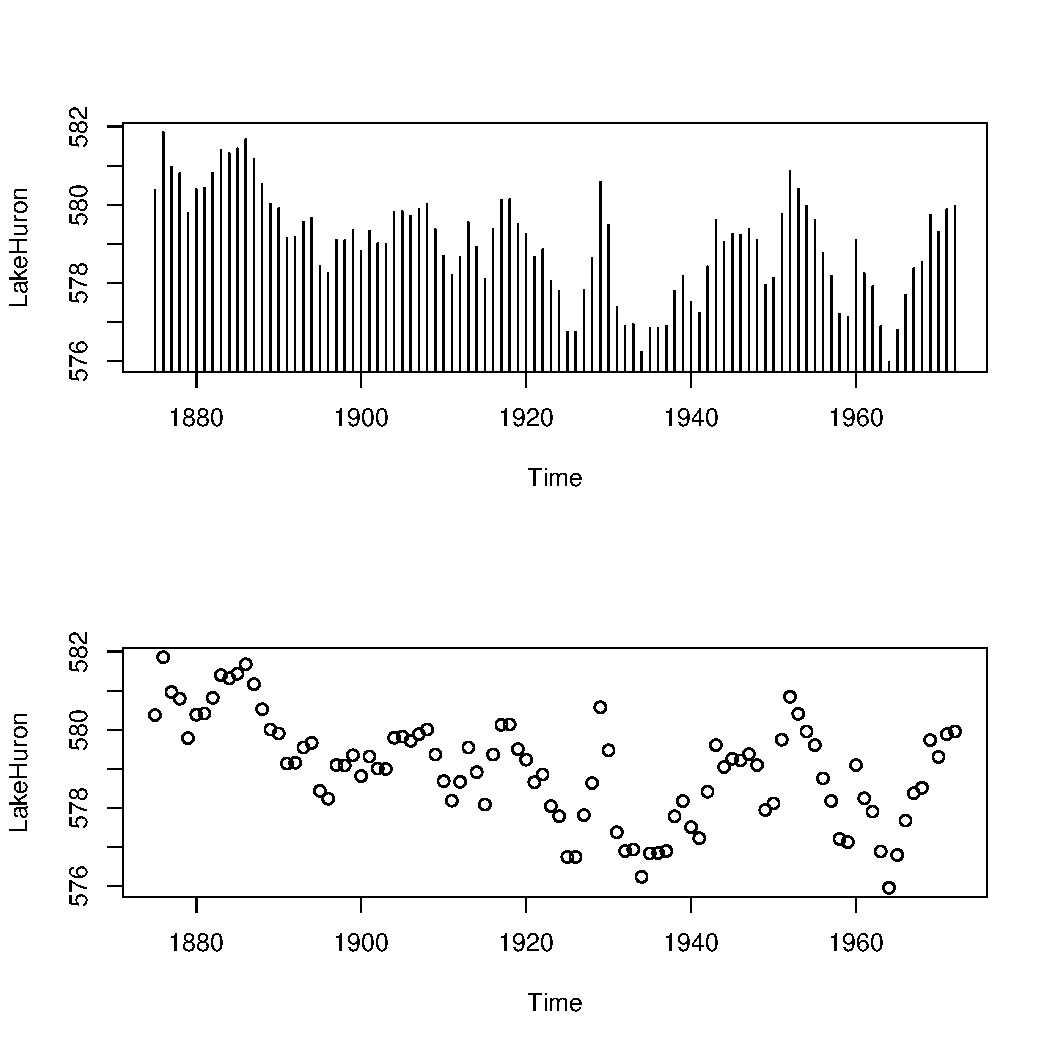
\includegraphics[width=5in, height=4in]{img/indpl-lakehuron.pdf}
    \caption{Index plots of the \texttt{LakeHuron} data}
    \label{fig:indpl-lakehuron}
  \end{figure}

\end{example}

\paragraph*{Density estimates}

Coming soon.
\subsection{Qualitative Data, Categorical Data, and Factors}
\label{sec-1-1-3}

\label{sub:Qualitative-Data}

Qualitative data are simply any type of data that are not numerical, or do not represent numerical quantities. Examples of qualitative variables include a subject's name, gender, race/ethnicity, political party, socioeconomic status, class rank, driver's license number, and social security number (SSN).

Please bear in mind that some data \emph{look} to be quantitative but are \emph{not}, because they do not represent numerical quantities and do not obey mathematical rules. For example, a person's shoe size is typically written with numbers: 8, or 9, or 12, or \(12\,\frac{1}{2}\). Shoe size is not quantitative, however, because if we take a size 8 and combine with a size 9 we do not get a size 17.

Some qualitative data serve merely to \emph{identify} the observation (such a subject's name, driver's license number, or SSN). This type of data does not usually play much of a role in statistics. But other qualitative variables serve to \emph{subdivide} the data set into categories; we call these \emph{factors}. In the above examples, gender, race, political party, and socioeconomic status would be considered factors (shoe size would be another one). The possible values of a factor are called its \emph{levels}. For instance, the factor \emph{gender} would have two levels, namely, male and female. Socioeconomic status typically has three levels: high, middle, and low.

Factors may be of two types: \emph{nominal}\index{nominal data} and \emph{ordinal}\index{ordinal data}. Nominal factors have levels that correspond to names of the categories, with no implied ordering. Examples of nominal factors would be hair color, gender, race, or political party. There is no natural ordering to ``Democrat'' and ``Republican''; the categories are just names associated with different groups of people. 

In contrast, ordinal factors have some sort of ordered structure to the underlying factor levels. For instance, socioeconomic status would be an ordinal categorical variable because the levels correspond to ranks associated with income, education, and occupation. Another example of ordinal categorical data would be class rank.

Factors have special status in \textsf{R}. They are represented internally by numbers, but even when they are written numerically their values do not convey any numeric meaning or obey any mathematical rules (that is, Stage III cancer is not Stage I cancer + Stage II cancer).

\begin{example}
The \texttt{state.abb}\index{Data sets!state.abb@\texttt{state.abb}}
vector gives the two letter postal abbreviations for all 50 states.


\begin{verbatim}
str(state.abb)
\end{verbatim}

\begin{verbatim}
  chr [1:50] "AL" "AK" "AZ" "AR" "CA" "CO" ...
\end{verbatim}

These would be ID data. The \texttt{state.name}\index{Data sets!state.name@\texttt{state.name}} vector lists all of the complete names and those data would also be ID.
\end{example}

\begin{example}
\textbf{U.S. State Facts and Features.} The U.S. Department of Commerce of the U.S. Census Bureau releases all sorts of information in the \emph{Statistical Abstract of the United States}, and the \texttt{state.region}\index{Data sets!state.region@\texttt{state.region}} data lists each of the 50 states and the region to which it belongs, be it Northeast, South, North Central, or West. See \texttt{?state.region}.


\begin{verbatim}
str(state.region)
state.region[1:5]
\end{verbatim}

\begin{verbatim}
  Factor w/ 4 levels "Northeast","South",..: 2 4 4 2 4 4 1 2 2 2 ...
 [1] South West  West  South West 
 Levels: Northeast South North Central West
\end{verbatim}

The \texttt{str}\index{str@\texttt{str}} output shows that \texttt{state.region} is already stored internally as a factor and it lists a couple of the factor levels. To see all of the levels we printed the first five entries of the vector in the second line.
\end{example}
\subsection{Displaying Qualitative Data}
\label{sec-1-1-4}

\label{sub:Displaying-Qualitative-Data}

\paragraph*{Tables}
\label{par:Tables}

One of the best ways to summarize qualitative data is with a table of the data values. We may count frequencies with the \texttt{table} function or list proportions with the \texttt{prop.table}\index{prop.table@\texttt{prop.table}} function (whose input is a frequency table). In the \textsf{R} Commander you can do it with \textsf{Statistics} \textsf{\(\triangleright\)} \textsf{Frequency Distribution}... Alternatively, to look at tables for all factors in the \texttt{Active data set}\index{Active data set@\texttt{Active data set}} you can do \textsf{Statistics} \textsf{\(\triangleright\)} \textsf{Summaries} \textsf{\(\triangleright\)} \textsf{Active Dataset}.


\begin{verbatim}
Tbl <- table(state.division)
\end{verbatim}


\begin{verbatim}
Tbl
\end{verbatim}

\begin{verbatim}
 state.division
        New England    Middle Atlantic     South Atlantic 
                  6                  3                  8 
 East South Central West South Central East North Central 
                  4                  4                  5 
 West North Central           Mountain            Pacific 
                  7                  8                  5
\end{verbatim}


\begin{verbatim}
Tbl/sum(Tbl)      # relative frequencies
\end{verbatim}

\begin{verbatim}
 state.division
        New England    Middle Atlantic     South Atlantic 
               0.12               0.06               0.16 
 East South Central West South Central East North Central 
               0.08               0.08               0.10 
 West North Central           Mountain            Pacific 
               0.14               0.16               0.10
\end{verbatim}


\begin{verbatim}
prop.table(Tbl)   # same thing
\end{verbatim}

\begin{verbatim}
 state.division
        New England    Middle Atlantic     South Atlantic 
               0.12               0.06               0.16 
 East South Central West South Central East North Central 
               0.08               0.08               0.10 
 West North Central           Mountain            Pacific 
               0.14               0.16               0.10
\end{verbatim}


\paragraph*{Bar Graphs}
\label{par:Bar-Graphs}

A bar graph is the analogue of a histogram for categorical data. A bar is displayed for each level of a factor, with the heights of the bars proportional to the frequencies of observations falling in the respective categories. A disadvantage of bar graphs is that the levels are ordered alphabetically (by default), which may sometimes obscure patterns in the display. 

\begin{example}
\textbf{U.S. State Facts and Features.} The \texttt{state.region} data lists each of the 50 states and the region to which it belongs, be it Northeast, South, North Central, or West. See \texttt{?state.region}. It is already stored internally as a factor. We make a bar graph with the \texttt{barplot}\index{barplot@\texttt{barplot}} function: 



\begin{verbatim}
barplot(table(state.region), cex.names = 0.50)
barplot(prop.table(table(state.region)), cex.names = 0.50)
\end{verbatim}

See Figure \ref{fig:bar-gr-stateregion}. The display on the left is a frequency bar graph because the \(y\) axis shows counts, while the display on the left is a relative frequency bar graph. The only difference between the two is the scale. Looking at the graph we see that the majority of the fifty states are in the South, followed by West, North Central, and finally Northeast. Over 30\% of the states are in the South.

Notice the \texttt{cex.names}\index{cex.names@\texttt{cex.names}} argument that we used, above. It shrinks the names on the \(x\) axis by 50\% which makes them easier to read. See \texttt{?par}\index{par@\texttt{par}} for a detailed list of additional plot parameters.






\begin{figure}[ht!]
    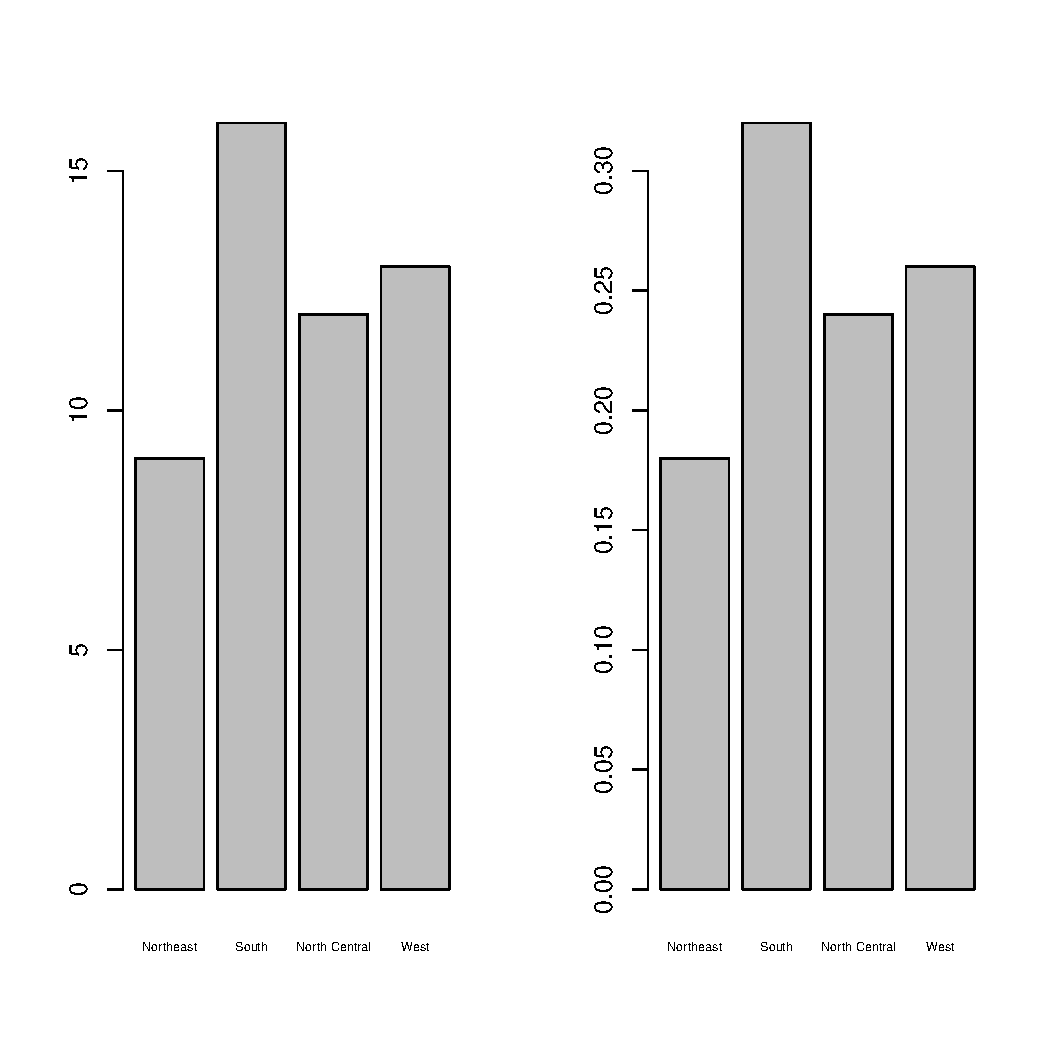
\includegraphics[width=5in, height=4in]{img/bar-gr-stateregion.pdf}
    \caption[Bar graphs of the \texttt{state.region} data]{\small The left graph is a frequency barplot made with \texttt{table} and the right is a relative frequency barplot made with \texttt{prop.table}.}
    \label{fig:bar-gr-stateregion}
  \end{figure}

\end{example}



\paragraph*{Pareto Diagrams}
\label{par:Pareto-Diagrams}

A pareto diagram is a lot like a bar graph except the bars are rearranged such that they decrease in height going from left to right. The rearrangement is handy because it can visually reveal structure (if any) in how fast the bars decrease -- this is much more difficult when the bars are jumbled. 

\begin{example}
\textbf{U.S. State Facts and Features.} The \texttt{state.division}\index{Data sets!state.division@\texttt{state.division}} data record the division (New England, Middle Atlantic, South Atlantic, East South Central, West South Central, East North Central, West North Central, Mountain, and Pacific) of the fifty states. We can make a pareto diagram with either the \texttt{RcmdrPlugin.IPSUR}\index{R packages@\textsf{R} packages!RcmdrPlugin.IPSUR@\texttt{RcmdrPlugin.IPSUR}} package or with the \texttt{pareto.chart}\index{pareto.chart@\texttt{pareto.chart}} function from the \texttt{qcc}\index{R packages@\textsf{R} packages!qcc@\texttt{qcc}} package \cite{qcc}. See Figure \ref{fig:Pareto-chart}. The code follows.



\begin{verbatim}
library(qcc)
pareto.chart(table(state.division), ylab="Frequency")
\end{verbatim}



\begin{figure}[ht!]
    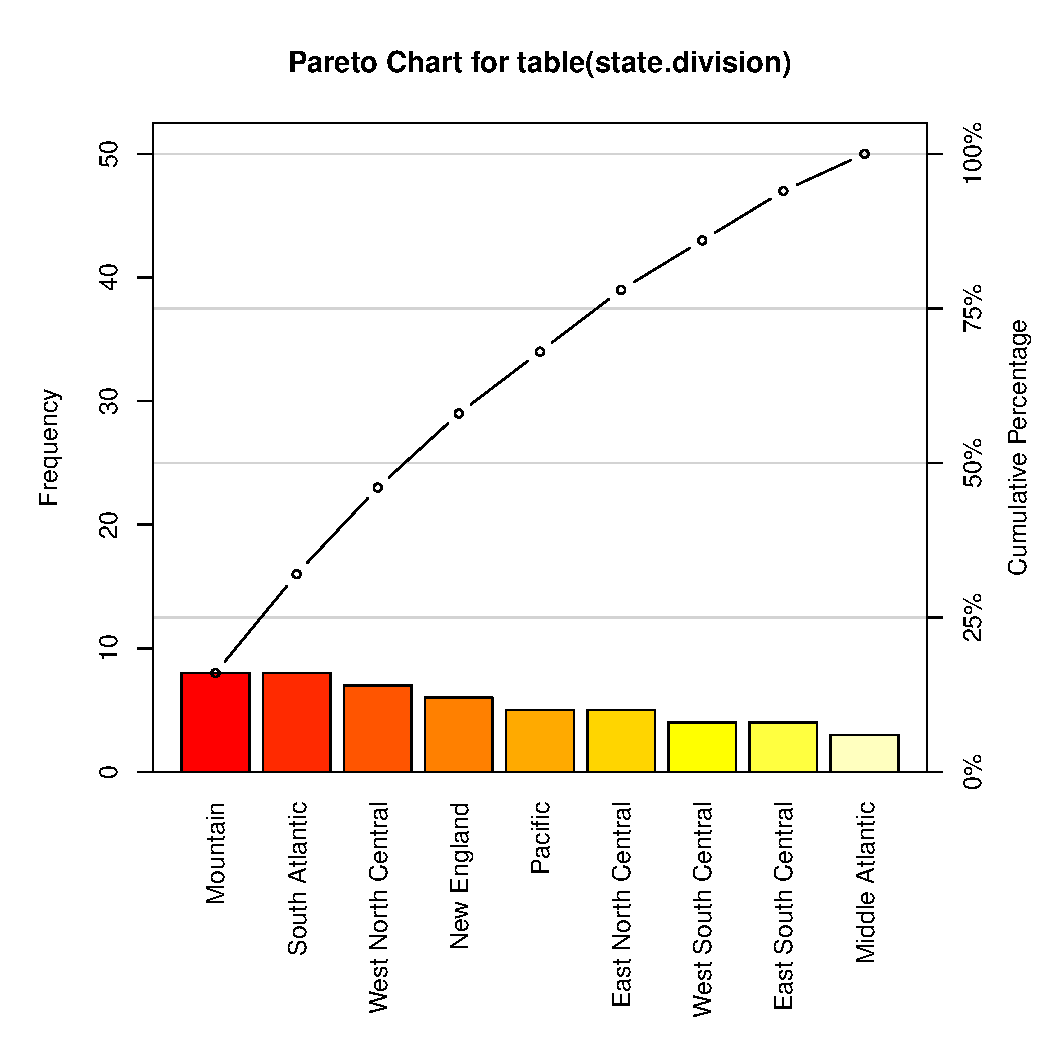
\includegraphics[width=5in, height=4in]{img/Pareto-chart.pdf}
    \caption{Pareto chart of the \texttt{state.division} data}
    \label{fig:Pareto-chart}
  \end{figure}

\end{example}



\paragraph*{Dot Charts}
\label{par:Dotcharts}

These are a lot like a bar graph that has been turned on its side with the bars replaced by dots on horizontal lines. They do not convey any more (or less) information than the associated bar graph, but the strength lies in the economy of the display. Dot charts are so compact that it is easy to graph very complicated multi-variable interactions together in one graph. See Section \ref{sec:Comparing-Data-Sets}. We will give an example here using the same data as above for comparison. The graph was produced by the following code.

\begin{example}


\begin{verbatim}
x <- table(state.region)
dotchart(as.vector(x), labels = names(x))
\end{verbatim}



\begin{figure}[ht!]
    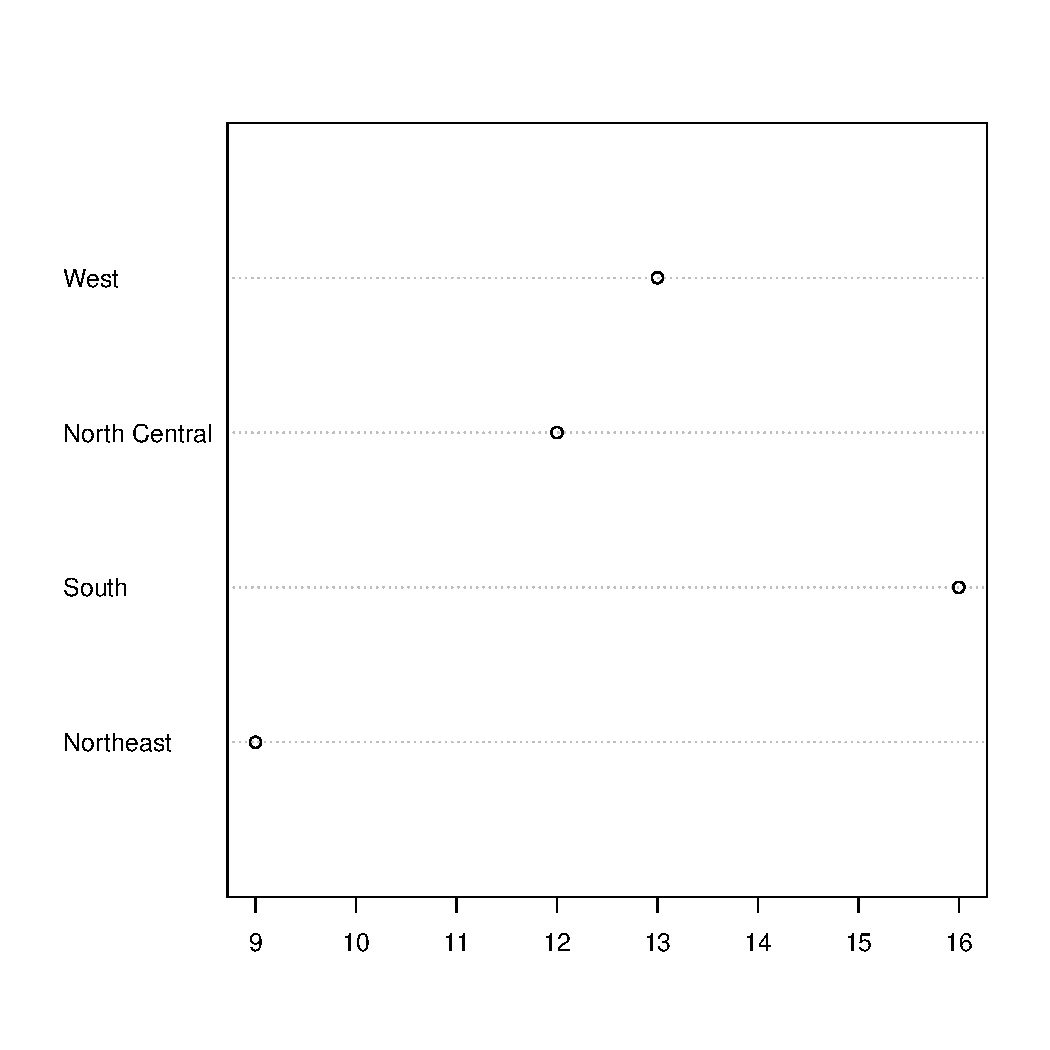
\includegraphics[width=5in, height=4in]{img/dot-charts.pdf}
    \caption{Dot chart of the \texttt{state.region} data}
    \label{fig:dot-charts}
  \end{figure}

See Figure \ref{fig:dot-charts}. Compare it to Figure \ref{fig:bar-gr-stateregion}.

\end{example}

\paragraph*{Pie Graphs}
\label{par:Pie-Graphs}

These can be done with \textsf{R} and the \textsf{R} Commander, but they fallen out of favor in recent years because researchers have determined that while the human eye is good at judging linear measures, it is notoriously bad at judging relative areas (such as those displayed by a pie graph). Pie charts are consequently a very bad way of displaying information. A bar chart or dot chart is a preferable way of displaying qualitative data. See \texttt{?pie}\index{pie@\texttt{pie}} for more information.

We are not going to do any examples of a pie graph and discourage their use elsewhere. 
\subsection{Logical Data}
\label{sec-1-1-5}

\label{sub:Logical-Data}

There is another type of information recognized by \textsf{R} which does not fall into the above categories. The value is either \texttt{TRUE} or \texttt{FALSE} (note that equivalently you can use \texttt{1 = TRUE}, \texttt{0 = FALSE}). Here is an example of a logical vector:


\begin{verbatim}
x <- 5:9
y <- (x < 7.3)
y
\end{verbatim}

\begin{verbatim}
 [1]  TRUE  TRUE  TRUE FALSE FALSE
\end{verbatim}

Many functions in \textsf{R} have options that the user may or may not want to activate in the function call. For example, the \texttt{stem.leaf} function has the \texttt{depths} argument which is \texttt{TRUE} by default. We saw in Section \ref{sub:Quantitative-Data} how to turn the option off, simply enter \texttt{stem.leaf(x, depths = FALSE)} and they will not be shown on the display.

We can swap \texttt{TRUE} with \texttt{FALSE} with the exclamation point \texttt{!}.


\begin{verbatim}
!y
\end{verbatim}

\begin{verbatim}
 [1] FALSE FALSE FALSE  TRUE  TRUE
\end{verbatim}
\subsection{Missing Data}
\label{sec-1-1-6}

\label{sub:Missing-Data}

Missing data are a persistent and prevalent problem in many statistical analyses, especially those associated with the social sciences. \textsf{R} reserves the special symbol \texttt{NA} to representing missing data.

Ordinary arithmetic with \texttt{NA} values give \texttt{NA}'s (addition, subtraction, \emph{etc}.) and applying a function to a vector that has an \texttt{NA} in it will usually give an \texttt{NA}.


\begin{verbatim}
x <- c(3, 7, NA, 4, 7)
y <- c(5, NA, 1, 2, 2)
x + y
\end{verbatim}

\begin{verbatim}
 [1]  8 NA NA  6  9
\end{verbatim}

Some functions have a \texttt{na.rm} argument which when \texttt{TRUE} will ignore missing data as if they were not there (such as \texttt{mean}, \texttt{var}, \texttt{sd}, \texttt{IQR}, \texttt{mad}, \ldots{}). 


\begin{verbatim}
sum(x)
sum(x, na.rm = TRUE)
\end{verbatim}

\begin{verbatim}
 [1] NA
 [1] 21
\end{verbatim}

Other functions do not have a \texttt{na.rm} argument and will return \texttt{NA} or an error if the argument has \texttt{NA}s. In those cases we can find the locations of any \texttt{NA}s with the \texttt{is.na} function and remove those cases with the \texttt{[]} operator.


\begin{verbatim}
is.na(x)
z <- x[!is.na(x)]
sum(z)
\end{verbatim}

\begin{verbatim}
 [1] FALSE FALSE  TRUE FALSE FALSE
 [1] 21
\end{verbatim}

The analogue of \texttt{is.na} for rectangular data sets (or data frames) is the \texttt{complete.cases} function. See Appendix \ref{sec:Editing-Data-Sets}.
\subsection{Other Data Types}
\label{sec-1-1-7}

\label{sub:other-data-types}
\section{Features of Data Distributions}
\label{sec-1-2}

\label{sec:features-of-data}

Given that the data have been appropriately displayed, the next step is to try to identify salient features represented in the graph. The acronym to remember is \emph{C}enter, \emph{U}nusual features, \emph{S}pread, and \emph{S}hape. (CUSS).
\subsection{Center}
\label{sec-1-2-1}

\label{sub:Center}

One of the most basic features of a data set is its center. Loosely speaking, the center of a data set is associated with a number that represents a middle or general tendency of the data. Of course, there are usually several values that would serve as a center, and our later tasks will be focused on choosing an appropriate one for the data at hand. Judging from the histogram that we saw in Figure \ref{fig:histograms-bins}, a measure of center would be about \(  35 \). 
\subsection{Spread}
\label{sec-1-2-2}

\label{sub:Spread}

The spread of a data set is associated with its variability; data sets with a large spread tend to cover a large interval of values, while data sets with small spread tend to cluster tightly around a central value. 
\subsection{Shape}
\label{sec-1-2-3}

\label{sub:Shape}

When we speak of the \emph{shape} of a data set, we are usually referring to the shape exhibited by an associated graphical display, such as a histogram. The shape can tell us a lot about any underlying structure to the data, and can help us decide which statistical procedure we should use to analyze them.

\paragraph*{Symmetry and Skewness}

A distribution is said to be \emph{right-skewed} (or \emph{positively skewed}) if the right tail seems to be stretched from the center. A \emph{left-skewed} (or \emph{negatively skewed}) distribution is stretched to the left side. A symmetric distribution has a graph that is balanced about its center, in the sense that half of the graph may be reflected about a central line of symmetry to match the other
half.

We have already encountered skewed distributions: both the discoveries data in Figure \ref{fig:stripcharts} and the \texttt{precip} data in Figure \ref{fig:histograms-bins} appear right-skewed. The \texttt{UKDriverDeaths} data in Example \ref{exa:-ukdriverdeaths-first} is relatively symmetric (but note the one extreme value 2654 identified at the bottom of the stemplot).

\paragraph*{Kurtosis}

Another component to the shape of a distribution is how ``peaked'' it is. Some distributions tend to have a flat shape with thin tails. These are called \emph{platykurtic}, and an example of a platykurtic distribution is the uniform distribution; see Section \ref{sec:The-Continuous-Uniform}. On the other end of the spectrum are distributions with a steep peak, or spike, accompanied by heavy tails; these are called \emph{leptokurtic}. Examples of leptokurtic distributions are the Laplace distribution and the logistic distribution. See Section \ref{sec:Other-Continuous-Distributions}. In between are distributions (called \emph{mesokurtic}) with a rounded peak and moderately sized tails. The standard example of a mesokurtic distribution is the famous bell-shaped curve, also known as the Gaussian, or normal, distribution, and the binomial distribution can be mesokurtic for specific choices of \(p\). See Sections \ref{sec:binom-dist} and \ref{sec:The-Normal-Distribution}.
\subsection{Clusters and Gaps}
\label{sec-1-2-4}

\label{sub:clusters-and-gaps}

Clusters or gaps are sometimes observed in quantitative data distributions. They indicate clumping of the data about distinct values, and gaps may exist between clusters. Clusters often suggest an underlying grouping to the data. For example, take a look at the \texttt{faithful} data which contains the duration of \texttt{eruptions} and the \texttt{waiting} time between eruptions of the Old Faithful geyser in Yellowstone National Park. Do not be frightened by the complicated information at the left of the display for now; we will learn how to interpret it in Section \ref{sec:Exploratory-Data-Analysis}.


\begin{verbatim}
library(aplpack)
with(faithful, stem.leaf(eruptions))
\end{verbatim}


\begin{verbatim}
[1] 35
1 | 2: represents 1.2
 leaf unit: 0.1
            n: 272
   12     s | 667777777777
   51    1. | 888888888888888888888888888899999999999
   71    2* | 00000000000011111111
   87     t | 2222222222333333
   92     f | 44444
   94     s | 66
   97    2. | 889
   98    3* | 0
  102     t | 3333
  108     f | 445555
  118     s | 6666677777
  (16)   3. | 8888888889999999
  138    4* | 0000000000000000111111111111111
  107     t | 22222222222233333333333333333
   78     f | 44444444444445555555555555555555555
   43     s | 6666666666677777777777
   21    4. | 88888888888899999
    4    5* | 0001
\end{verbatim}

There are definitely two clusters of data here; an upper cluster and a lower cluster. 
\subsection{Extreme Observations and other Unusual Features}
\label{sec-1-2-5}

\label{sub:Extreme-Observations-and}

Extreme observations fall far from the rest of the data. Such observations are troublesome to many statistical procedures; they cause exaggerated estimates and instability. It is important to identify extreme observations and examine the source of the data more closely. There are many possible reasons underlying an extreme observation:

\begin{itemize}
\item \textbf{Maybe the value is a typographical error.} Especially with large data sets becoming more prevalent, many of which being recorded by hand, mistakes are a common problem. After closer scrutiny, these can often be fixed.
\item \textbf{Maybe the observation was not meant for the study}, because it does not belong to the population of interest. For example, in medical research some subjects may have relevant complications in their genealogical history that would rule out their participation in the experiment. Or when a manufacturing company investigates the properties of one of its devices, perhaps a particular product is malfunctioning and is not representative of the majority of the items.
\item \textbf{Maybe it indicates a deeper trend or phenomenon.} Many of the most influential scientific discoveries were made when the investigator noticed an unexpected result, a value that was not predicted by the classical theory. Albert Einstein, Louis Pasteur, and others built their careers on exactly this circumstance.
\end{itemize}
\section{Descriptive Statistics}
\label{sec-1-3}

\label{sec:Descriptive-Statistics}
\subsection{Frequencies and Relative Frequencies}
\label{sec-1-3-1}

\label{sub:Frequencies-and-Relative}

These are used for categorical data. The idea is that there are a number of different categories, and we would like to get some idea about how the categories are represented in the population. 
\subsection{Measures of Center}
\label{sec-1-3-2}

\label{sub:Measures-of-Center}

The \emph{sample mean} is denoted \(\overline{x}\) (read ``\(x\)-bar'') and is simply the arithmetic average of the observations:

\begin{equation} 
\overline{x}=\frac{x_{1}+x_{2}+\cdots+x_{n}}{n}=\frac{1}{n}\sum_{i=1}^{n}x_{i}.
\end{equation}

\begin{itemize}
\item Good: natural, easy to compute, has nice mathematical properties
\item Bad: sensitive to extreme values
\end{itemize}

It is appropriate for use with data sets that are not highly skewed without extreme observations.

The \emph{sample median} is another popular measure of center and is denoted \(\tilde{x}\). To calculate its value, first sort the data into an increasing sequence of numbers. If the data set has an odd number of observations then \(\tilde{x}\) is the value of the middle observation, which lies in position \((n+1)/2\); otherwise, there are two middle observations and \(\tilde{x}\) is the average of those middle values.

\begin{itemize}
\item Good: resistant to extreme values, easy to describe
\item Bad: not as mathematically tractable, need to sort the data to calculate
\end{itemize}

One desirable property of the sample median is that it is \emph{resistant} to extreme observations, in the sense that the value of \(\tilde{x}\) depends only on those data values in the middle, and is quite unaffected by the actual values of the outer observations in the ordered list. The same cannot be said for the sample mean. Any significant changes in the magnitude of an observation \(x_{k}\) results in a corresponding change in the value of the mean. Consequently, the sample mean is said to be \emph{sensitive} to extreme observations.

The \emph{trimmed mean} is a measure designed to address the sensitivity of the sample mean to extreme observations. The idea is to ``trim'' a fraction (less than 1/2) of the observations off each end of the ordered list, and then calculate the sample mean of what remains. We will denote it by \(\overline{x}_{t=0.05}\).

\begin{itemize}
\item Good: resistant to extreme values, shares nice statistical properties
\item Bad: need to sort the data
\end{itemize}


\paragraph*{How to do it with \textsf{R}}

\begin{itemize}
\item You can calculate frequencies or relative frequencies with the \texttt{table} function, and relative frequencies with \texttt{prop.table(table())}. \item You can calculate the sample mean of a data vector \texttt{x} with the command \texttt{mean(x)}.
\item You can calculate the sample median of \texttt{x} with the command \texttt{median(x)}. \item You can calculate the trimmed mean with the \texttt{trim} argument; \texttt{mean(x, trim = 0.05)}.
\end{itemize}
\subsection{Order Statistics and the Sample Quantiles}
\label{sec-1-3-3}

\label{sub:Order-Statistics-and}

A common first step in an analysis of a data set is to sort the values. Given a data set \(x_{1}\), \(x_{2}\), \ldots{}, \(x_{n}\), we may sort the values to obtain an increasing sequence

\begin{equation} 
x_{(1)}\leq x_{(2)}\leq x_{(3)}\leq\cdots\leq x_{(n)}
\end{equation}

and the resulting values are called the \emph{order statistics}. The \(k^{\mathrm{th}}\) entry in the list, \(x_{(k)}\), is the \(k^{\mathrm{th}}\) order statistic, and approximately \(100(k/n)\)\% of the observations fall below \(x_{(k)}\). The order statistics give an indication of the shape of the data distribution, in the sense that a person can look at the order statistics and have an idea about where the data are concentrated, and where they are sparse.

The \emph{sample quantiles} are related to the order statistics. Unfortunately, there is not a universally accepted definition of them. Indeed, \textsf{R} is equipped to calculate quantiles using nine distinct definitions! We will describe the default method (\texttt{type = 7}), but the interested reader can see the details for the other methods with \texttt{?quantile}.

Suppose the data set has \(n\) observations. Find the sample quantile of order \(p\) (\(0<p<1\)), denoted \(\tilde{q}_{p}\) , as follows: 

\begin{description}
\item[First step:] sort the data to obtain the order statistics \(x_{(1)}\), \(x_{(2)}\), \ldots{},\(x_{(n)}\).
\item[Second step:] calculate \((n-1)p+1\) and write it in the form \(k.d\), where \(k\) is an integer and \(d\) is a decimal.
\item[Third step:] The sample quantile \(\tilde{q}_{p}\) is
   \begin{equation}
      \tilde{q}_{p}=x_{(k)}+d(x_{(k+1)}-x_{(k)}).
   \end{equation}
\end{description}


The interpretation of \(\tilde{q}_{p}\) is that approximately \(100p\) \% of the data fall below the value \(\tilde{q}_{p}\) . 

Keep in mind that there is not a unique definition of percentiles, quartiles, \emph{etc}. Open a different book, and you'll find a different definition. The difference is small and seldom plays a role except in small data sets with repeated values. In fact, most people do not even notice in common use.

Clearly, the most popular sample quantile is \(\tilde{q}_{0.50}\), also known as the sample median, \(\tilde{x}\). The closest runners-up are the \emph{first quartile} \(\tilde{q}_{0.25}\) and the \emph{third quartile} \(\tilde{q}_{0.75}\) (the \emph{second quartile} is the median). 


\paragraph*{How to do it with \textsf{R}}

\subparagraph*{At the command prompt}
we can find the order statistics of a data set stored in a vector \texttt{x} with the command \texttt{sort(x)}.

We can calculate the sample quantiles of any order \(p\) where \(0<p<1\) for a data set stored in a data vector \texttt{x} with the \texttt{quantile} function, for instance, the command \texttt{quantile(x, probs = c(0, 0.25, 0.37))} will return the smallest observation, the first quartile, \(\tilde{q}_{0.25}\), and the 37th sample quantile, \(\tilde{q}_{0.37}\). For \(\tilde{q}_{p}\) simply change the values in the \texttt{probs} argument to the value \(p\).


\subparagraph*{With the \textsf{R} Commander}
we can find the order statistics of a variable in the \texttt{Active data set} by doing \textsf{Data \(\triangleright\) Manage variables in Active data set ... \(\triangleright\) Compute new variable}.\ldots{} In the \textsf{Expression to compute} dialog simply type \texttt{sort(varname)}, where \texttt{varname} is the variable that it is desired to sort.

In \texttt{Rcmdr}, we can calculate the sample quantiles for a particular variable with the sequence \textsf{Statistics \(\triangleright\) Summaries \(\triangleright\) Numerical Summaries}... We can automatically calculate the quartiles for all variables in the \texttt{Active data set} with the sequence \textsf{Statistics \(\triangleright\) Summaries \(\triangleright\) Active Dataset}.
\subsection{Measures of Spread}
\label{sec-1-3-4}

\label{sub:Measures-of-Spread}

\paragraph*{Sample Variance and Standard Deviation}

The \emph{sample variance} is denoted \(s^{2}\) and is calculated with the formula

\begin{equation}
s^{2}=\frac{1}{n-1}\sum_{i=1}^{n}(x_{i}-\overline{x})^{2}.
\end{equation}

The \emph{sample standard deviation} is \(s=\sqrt{s^{2}}\). Intuitively, the sample variance is approximately the average squared distance of the observations from the sample mean. The sample standard deviation is used to scale the estimate back to the measurement units of the original data.

\begin{itemize}
\item Good: tractable, has nice mathematical/statistical properties
\item Bad: sensitive to extreme values
\end{itemize}

We will spend a lot of time with the variance and standard deviation in the coming chapters. In the meantime, the following two rules give some meaning to the standard deviation, in that there are bounds on how much of the data can fall past a certain distance from the mean.

\begin{fact}
Chebychev's Rule: The proportion of observations within \(k\) standard deviations of the mean is at least \(1-1/k^{2}\), \emph{i.e.}, at least 75\%, 89\%, and 94\% of the data are within 2, 3, and 4 standard deviations of the mean, respectively.
\end{fact}

Note that Chebychev's Rule does not say anything about when \(k=1\), because \(1-1/1^{2}=0\), which states that at least 0\% of the observations are within one standard deviation of the mean (which is not saying much).

Chebychev's Rule applies to any data distribution, \emph{any} list of numbers, no matter where it came from or what the histogram looks like. The price for such generality is that the bounds are not very tight; if we know more about how the data are shaped then we can say more about how much of the data can fall a given distance from the mean.

\begin{fact}
\label{fac:Empirical-Rule}Empirical Rule: If data follow a bell-shaped
curve, then approximately 68\%, 95\%, and 99.7\% of the data are within
1, 2, and 3 standard deviations of the mean, respectively. 
\end{fact}


\paragraph*{Interquartile Range}

Just as the sample mean is sensitive to extreme values, so the associated measure of spread is similarly sensitive to extremes. Further, the problem is exacerbated by the fact that the extreme distances are squared. We know that the sample quartiles are resistant to extremes, and a measure of spread associated with them is the \emph{interquartile range} (\(IQR\)) defined by \(IQR=q_{0.75}-q_{0.25}\).

\begin{itemize}
\item Good: stable, resistant to outliers, robust to nonnormality, easy to explain
\item Bad: not as tractable, need to sort the data, only involves the middle 50\% of the data.
\end{itemize}

\paragraph*{Median Absolute Deviation}

A measure even more robust than the \(IQR\) is the \emph{median absolute deviation} (\(MAD\)). To calculate it we first get the median \(\widetilde{x}\), next the \emph{absolute deviations} \(|x_{1}-\tilde{x}|\), \(|x_{2}-\tilde{x}|\), \ldots{}, \(|x_{n}-\tilde{x}|\), and the \(MAD\) is proportional to the median of those deviations:

\begin{equation}
MAD\propto\mbox{median}(|x_{1}-\tilde{x}|,\ |x_{2}-\tilde{x}|,\ldots,|x_{n}-\tilde{x}|).
\end{equation}

That is, the \(MAD=c\cdot\mbox{median}(|x_{1}-\tilde{x}|,\ |x_{2}-\tilde{x}|,\ldots,|x_{n}-\tilde{x}|)\), where \(c\) is a constant chosen so that the \(MAD\) has nice properties. The value of \(c\) in \textsf{R} is by default \(c=1.4286\). This value is chosen to ensure that the estimator of \(\sigma\) is correct, on the average, under suitable sampling assumptions (see Section \ref{sec:Point-Estimation-1}).

\begin{itemize}
\item Good: stable, very robust, even more so than the \(IQR\).
\item Bad: not tractable, not well known and less easy to explain.
\end{itemize}


\paragraph*{Comparing Apples to Apples}

We have seen three different measures of spread which, for a given data set, will give three different answers. Which one should we use? It depends on the data set. If the data are well behaved, with an approximate bell-shaped distribution, then the sample mean and sample standard deviation are natural choices with nice mathematical properties. However, if the data have an unusual or skewed shape with several extreme values, perhaps the more resistant choices among the \(IQR\) or \(MAD\) would be more appropriate.

However, once we are looking at the three numbers it is important to understand that the estimators are not all measuring the same quantity, on the average. In particular, it can be shown that when the data follow an approximately bell-shaped distribution, then on the average, the sample standard deviation \(s\) and the \(MAD\) will be the approximately the same value, namely, \(\sigma\), but the \(IQR\) will be on the average 1.349 times larger than \(s\) and the \(MAD\). See \ref{cha:Sampling-Distributions} for more details.


\paragraph*{How to do it with \textsf{R}}

\subparagraph*{At the command prompt}
we may compute the sample range with \texttt{range(x)} and the sample variance with \texttt{var(x)}, where \texttt{x} is a numeric vector. The sample standard deviation is \texttt{sqrt(var(x))} or just \texttt{sd(x)}. The \(IQR\) is \texttt{IQR(x)} and the median absolute deviation is \texttt{mad(x)}.

\subparagraph*{With the \textsf{R} Commander}
we can calculate the sample standard deviation with the \textsf{Statistics \(\triangleright\) Summaries \(\triangleright\) Numerical Summaries}... combination. \textsf{R} Commander does not calculate the \(IQR\) or \(MAD\) in any of the menu selections, by default.
\subsection{Measures of Shape \label{sub:Measures-of-Shape}}
\label{sec-1-3-5}


\paragraph*{Sample Skewness}

The \emph{sample skewness}, denoted by \(g_{1}\), is defined by the formula

\begin{equation}
g_{1}=\frac{1}{n}\frac{\sum_{i=1}^{n}(x_{i}-\overline{x})^{3}}{s^{3}}.
\end{equation}

The sample skewness can be any value \(-\infty<g_{1}<\infty\). The sign of \(g_{1}\) indicates the direction of skewness of the distribution. Samples that have \(g_{1}>0\) indicate right-skewed distributions (or positively skewed), and samples with \(g_{1}<0\) indicate left-skewed distributions (or negatively skewed). Values of \(g_{1}\) near zero indicate a symmetric distribution. These are not hard and fast rules, however. The value of \(g_{1}\) is subject to sampling variability and thus only provides a suggestion to the skewness of the underlying distribution. 

We still need to know how big is ``big'', that is, how do we judge whether an observed value of \(g_{1}\) is far enough away from zero for the data set to be considered skewed to the right or left? A good rule of thumb is that data sets with skewness larger than \(2\sqrt{6/n}\) in magnitude are substantially skewed, in the direction of the sign of \(g_{1}\). See Tabachnick \& Fidell \cite{Tabachnick2006} for details.

\paragraph*{Sample Excess Kurtosis}

The \emph{sample excess kurtosis}, denoted by \(g_{2}\), is given by the formula

\begin{equation}
g_{2}=\frac{1}{n}\frac{\sum_{i=1}^{n}(x_{i}-\overline{x})^{4}}{s^{4}}-3.
\end{equation}

The sample excess kurtosis takes values \(-2\leq g_{2}<\infty\). The subtraction of 3 may seem mysterious but it is done so that mound shaped samples have values of \(g_{2}\) near zero. Samples with \(g_{2}>0\) are called \emph{leptokurtic}, and samples with \(g_{2}<0\) are called \emph{platykurtic}. Samples with \(g_{2}\approx0\) are called \emph{mesokurtic}.

As a rule of thumb, if \(|g_{2}|>4\sqrt{6/n}\) then the sample excess kurtosis is substantially different from zero in the direction of the sign of \(g_{2}\). See Tabachnick \& Fidell \cite{Tabachnick2006} for details.

Notice that both the sample skewness and the sample kurtosis are invariant with respect to location and scale, that is, the values of \(g_{1}\) and \(g_{2}\) do not depend on the measurement units of the data. 

\paragraph*{How to do it with \textsf{R}}

The \texttt{e1071} package \cite{Dimitriadoue1071} has the \texttt{skewness} function for the sample skewness and the \texttt{kurtosis} function for the sample excess kurtosis. Both functions have a \texttt{na.rm} argument which is \texttt{FALSE} by default.

\begin{example}
We said earlier that the \texttt{discoveries} data looked positively skewed; let's see what the statistics say:
\end{example}


\begin{verbatim}
library(e1071)
skewness(discoveries)
2*sqrt(6/length(discoveries))
\end{verbatim}

\begin{verbatim}
 [1] 1.2076
 [1] 0.4898979
\end{verbatim}

The data are definitely skewed to the right. Let us check the sample excess kurtosis of the \texttt{UKDriverDeaths} data:


\begin{verbatim}
kurtosis(UKDriverDeaths)
4*sqrt(6/length(UKDriverDeaths))
\end{verbatim}

\begin{verbatim}
 [1] 0.07133848
 [1] 0.7071068
\end{verbatim}

so that the \texttt{UKDriverDeaths} data appear to be mesokurtic, or at least not substantially leptokurtic.
\section{Exploratory Data Analysis}
\label{sec-1-4}

\label{sec:Exploratory-Data-Analysis}

This field was founded (mostly) by John Tukey (1915-2000). Its tools are useful when not much is known regarding the underlying causes associated with the data set, and are often used for checking assumptions. For example, suppose we perform an experiment and collect some data\ldots{} now what? We look at the data using exploratory visual tools.
\subsection{More About Stemplots}
\label{sec-1-4-1}


There are many bells and whistles associated with stemplots, and the \texttt{stem.leaf} function can do many of them.

\begin{description}
\item[Trim Outliers:] Some data sets have observations that fall far from the bulk of the other data (in a sense made more precise in Section \ref{sub:Outliers}). These extreme observations often obscure the underlying structure to the data and are best left out of the data display. The \texttt{trim.outliers} argument (which is \texttt{TRUE} by default) will separate the extreme observations from the others and graph the stemplot without them; they are listed at the bottom (respectively, top) of the stemplot with the label \texttt{HI} (respectively \texttt{LO}).
\item[Split Stems:] The standard stemplot has only one line per stem, which means that all observations with first digit \texttt{3} are plotted on the same line, regardless of the value of the second digit. But this gives some stemplots a ``skyscraper'' appearance, with too many observations stacked onto the same stem. We can often fix the display by increasing the number of lines available for a given stem. For example, we could make two lines per stem, say, \texttt{3*} and \texttt{3.}. Observations with second digit 0 through 4 would go on the upper line, while observations with second digit 5 through 9 would go on the lower line. (We could do a similar thing with five lines per stem, or even ten lines per stem.) The end result is a more spread out stemplot which often looks better. A good example of this was shown on page \pageref{exa:stemleaf-multiple-lines-stem}.
\item[Depths:] these are used to give insight into the balance of the observations as they accumulate toward the median. In a column beside the standard stemplot, the frequency of the stem containing the sample median is shown in parentheses. Next, frequencies are accumulated from the outside inward, including the outliers. Distributions that are more symmetric will have better balanced depths on either side of the sample median.
\end{description}


\paragraph*{How to do it with \textsf{R}}

The basic command is \texttt{stem(x)} or a more sophisticated version written by Peter Wolf called \texttt{stem.leaf(x)} in the \textsf{R} Commander. We will describe \texttt{stem.leaf} since that is the one used by \textsf{R} Commander.


WARNING: Sometimes when making a stem plot the result will not be what you expected. There are several reasons for this: 

\begin{itemize}
\item Stemplots by default will trim extreme observations (defined in Section \ref{sub:Outliers}) from the display. This in some cases will result in stemplots that are not as wide as expected.
\item The leafs digit is chosen automatically by \texttt{stem.leaf} according to an algorithm that the computer believes will represent the data well. Depending on the choice of the digit, \texttt{stem.leaf} may drop digits from the data or round the values in unexpected ways.
\end{itemize}

Let us take a look at the \texttt{rivers} data set\label{ite:stemplot-rivers}.


\begin{verbatim}
stem.leaf(rivers)
\end{verbatim}


\begin{verbatim}
1 | 2: represents 120
 leaf unit: 10
            n: 141
    1     1 | 3
   29     2 | 0111133334555556666778888899
   64     3 | 00000111122223333455555666677888999
  (18)    4 | 011222233344566679
   59     5 | 000222234467
   47     6 | 0000112235789
   34     7 | 12233368
   26     8 | 04579
   21     9 | 0008
   17    10 | 035
   14    11 | 07
   12    12 | 047
    9    13 | 0
HI: 1450 1459 1770 1885 2315 2348 2533 3710
\end{verbatim}

The stemplot shows a right-skewed shape to the \texttt{rivers} data distribution. Notice that the last digit of each of the data values were dropped from the display. Notice also that there were eight extreme observations identified by the computer, and their exact values are listed at the bottom of the stemplot. Look at the scale on the left of the stemplot and try to imagine how ridiculous the graph would have looked had we tried to include enough stems to include these other eight observations; the stemplot would have stretched over several pages. Notice finally that we can use the depths to approximate the sample median for these data. The median lies in the row identified by \texttt{(18)}, which means that the median is the average of the ninth and tenth observation on that row. Those two values correspond to \texttt{43} and \texttt{43}, so a good guess for the median would be 430. (For the record, the sample median is \(\widetilde{x}=425\). Recall that stemplots round the data to the nearest stem-leaf pair.) 

Next let us see what the \texttt{precip} data look like.


\begin{verbatim}
stem.leaf(precip)
\end{verbatim}


\begin{verbatim}
1 | 2: represents 12
 leaf unit: 1
            n: 70
LO: 7 7.2 7.8 7.8
    8    1* | 1344
   13    1. | 55677
   16    2* | 024
   18    2. | 59
   28    3* | 0000111234
  (15)   3. | 555566677788899
   27    4* | 0000122222334
   14    4. | 56688899
    6    5* | 44
    4    5. | 699
HI: 67
\end{verbatim}

Here is an example of split stems, with two lines per stem. The final digit of each datum has been dropped for the display. The data appear to be left skewed with four extreme values to the left and one extreme value to the right. The sample median is approximately 37 (it turns out to be 36.6).
\subsection{Hinges and the Five Number Summary}
\label{sec-1-4-2}

\label{sub:hinges-and-5NS}

Given a data set \(x_{1}\), \(x_{2}\), \ldots{}, \(x_{n}\), the hinges are found by the following method:  
\begin{itemize}
\item Find the order statistics \(x_{(1)}\), \(x_{(2)}\), \ldots{}, \(x_{(n)}\).
\item The \emph{lower hinge} \(h_{L}\) is in position \(L=\left\lfloor (n+3)/2\right\rfloor / 2\), where the symbol \( \left\lfloor x\right\rfloor \) denotes the largest integer less than or equal to \(x\). If the position \(L\) is not an integer, then the hinge \(h_{L}\) is the average of the adjacent order statistics.
\item The \emph{upper hinge} \(h_{U}\) is in position \(n+1-L\).
\end{itemize}
Given the hinges, the \emph{five number summary} (\(5NS\)) is 
\begin{equation} 
5NS=(x_{(1)},\ h_{L},\ \tilde{x},\ h_{U},\ x_{(n)}).
\end{equation}
An advantage of the \(5NS\) is that it reduces a potentially large data set to a shorter list of only five numbers, and further, these numbers give insight regarding the shape of the data distribution similar to the sample quantiles in Section \ref{sub:Order-Statistics-and}.

\paragraph*{How to do it with \textsf{R}}

If the data are stored in a vector \texttt{x}, then you can compute the \(5NS\) with the \texttt{fivenum} function.
\subsection{Boxplots}
\label{sec-1-4-3}

\label{sub:boxplots}

A boxplot is essentially a graphical representation of the \(5NS\). It can be a handy alternative to a stripchart when the sample size is large.

A boxplot is constructed by drawing a box alongside the data axis with sides located at the upper and lower hinges. A line is drawn parallel to the sides to denote the sample median. Lastly, whiskers are extended from the sides of the box to the maximum and minimum data values (more precisely, to the most extreme values that are not potential outliers, defined below).

Boxplots are good for quick visual summaries of data sets, and the relative positions of the values in the \(5NS\) are good at indicating the underlying shape of the data distribution, although perhaps not as effectively as a histogram. Perhaps the greatest advantage of a boxplot is that it can help to objectively identify extreme observations in the data set as described in the next section.

Boxplots are also good because one can visually assess multiple features of the data set simultaneously:

\begin{description}
\item[Center] can be estimated by the sample median, \(\tilde{x}\).
\item[Spread] can be judged by the width of the box, \(h_{U}-h_{L}\). We know that this will be close to the \(IQR\), which can be compared to \(s\) and the \(MAD\), perhaps after rescaling if appropriate.
\item[Shape] is indicated by the relative lengths of the whiskers, and the position of the median inside the box. Boxes with unbalanced whiskers indicate skewness in the direction of the long whisker. Skewed distributions often have the median tending in the opposite direction of skewness. Kurtosis can be assessed using the box and whiskers. A wide box with short whiskers will tend to be platykurtic, while a skinny box with wide whiskers indicates leptokurtic distributions.
\item[Extreme observations] are identified with open circles (see below).
\end{description}
\subsection{Outliers}
\label{sec-1-4-4}

\label{sub:Outliers}

A \emph{potential outlier} is any observation that falls beyond 1.5 times the width of the box on either side, that is, any observation less than \(h_{L}-1.5(h_{U}-h_{L})\) or greater than \(h_{U}+1.5(h_{U}-h_{L})\). A \emph{suspected outlier} is any observation that falls beyond 3 times the width of the box on either side. In \textsf{R}, both potential and suspected outliers (if present) are denoted by open circles; there is no distinction between the two. 

When potential outliers are present, the whiskers of the boxplot are then shortened to extend to the most extreme observation that is not a potential outlier. If an outlier is displayed in a boxplot, the index of the observation may be identified in a subsequent plot in \texttt{Rcmdr} by clicking the \textsf{Identify outliers with mouse} option in the \textsf{Boxplot} dialog.

What do we do about outliers? They merit further investigation. The primary goal is to determine why the observation is outlying, if possible. If the observation is a typographical error, then it should be corrected before continuing. If the observation is from a subject that does not belong to the population of interest, then perhaps the datum should be removed. Otherwise, perhaps the value is hinting at some hidden structure to the data.

\paragraph*{How to do it with \textsf{R}}

The quickest way to visually identify outliers is with a boxplot, described above. Another way is with the \texttt{boxplot.stats} function.

\begin{example}
The \texttt{rivers} data. We will look for potential outliers in the \texttt{rivers} data.


\begin{verbatim}
boxplot.stats(rivers)$out
\end{verbatim}

\begin{verbatim}
  [1] 1459 1450 1243 2348 3710 2315 2533 1306 1270 1885 1770
\end{verbatim}

We may change the \texttt{coef} argument to 3 (it is 1.5 by default) to identify suspected outliers.


\begin{verbatim}
boxplot.stats(rivers, coef = 3)$out
\end{verbatim}

\begin{verbatim}
 [1] 2348 3710 2315 2533 1885
\end{verbatim}

\end{example}
\subsection{Standardizing variables}
\label{sec-1-4-5}


It is sometimes useful to compare data sets with each other on a scale that is independent of the measurement units. Given a set of observed data \(x_{1}\), \(x_{2}\), \ldots{}, \(x_{n}\) we get \(z\) scores, denoted \(z_{1}\), \(z_{2}\), \ldots{}, \(z_{n}\), by means of the following formula

\[
z_{i}=\frac{x_{i}-\overline{x}}{s},\quad i=1,\,2,\,\ldots,\, n.
\]


\paragraph*{How to do it with \textsf{R}}

The \texttt{scale} function will rescale a numeric vector (or data frame) by subtracting the sample mean from each value (column) and/or by dividing each observation by the sample standard deviation.
\section{Multivariate Data and Data Frames}
\label{sec-1-5}

\label{sec:multivariate-data}

We have had experience with vectors of data, which are long lists of numbers. Typically, each entry in the vector is a single measurement on a subject or experimental unit in the study. We saw in Section \ref{sub:Vectors} how to form vectors with the \texttt{c} function or the \texttt{scan} function. 

However, statistical studies often involve experiments where there are two (or more) measurements associated with each subject. We display the measured information in a rectangular array in which each row corresponds to a subject, and the columns contain the measurements for each respective variable. For instance, if one were to measure the height and weight and hair color of each of 11 persons in a research study, the information could be represented with a rectangular array. There would be 11 rows. Each row would have the person's height in the first column and hair color in the second column.

The corresponding objects in \textsf{R} are called \emph{data frames}, and they can be constructed with the \texttt{data.frame} function. Each row is an observation, and each column is a variable.

\begin{example}
Suppose we have two vectors \texttt{x} and \texttt{y} and we want to make a data frame out of them.


\begin{verbatim}
x <- 5:8
y <- letters[3:6]
A <- data.frame(v1 = x, v2 = y)
\end{verbatim}

\end{example}

Notice that \texttt{x} and \texttt{y} are the same length. This is \emph{necessary}. Also notice that \texttt{x} is a numeric vector and \texttt{y} is a character vector. We may choose numeric and character vectors (or even factors) for the columns of the data frame, but each column must be of exactly one type. That is, we can have a column for \texttt{height} and a column for \texttt{gender}, but we will get an error if we try to mix function \texttt{height} (numeric) and \texttt{gender} (character or factor) information in the same column.

Indexing of data frames is similar to indexing of vectors. To get the entry in row \(i\) and column \(j\) do \texttt{A[i,j]}. We can get entire rows and columns by omitting the other index. 


\begin{verbatim}
A[3,]
A[1, ]
A[ ,2]
\end{verbatim}

\begin{verbatim}
   v1 v2
 3  7  e
   v1 v2
 1  5  c
 [1] c d e f
 Levels: c d e f
\end{verbatim}

There are several things happening above. Notice that \texttt{A[3,]} gave a data frame (with the same entries as the third row of \texttt{A}) yet \texttt{A[1, ]} is a numeric vector. \texttt{A[ ,2]} is a factor vector because the default setting for \texttt{data.frame} is \texttt{stringsAsFactors = TRUE}.

Data frames have a \texttt{names} attribute and the names may be extracted with the \texttt{names} function. Once we have the names we may extract given columns by way of the dollar sign.


\begin{verbatim}
names(A)
A$v1
\end{verbatim}

\begin{verbatim}
 [1] "v1" "v2"
 [1] 5 6 7 8
\end{verbatim}

The above is identical to \texttt{A[ ,1]}. 
\subsection{Bivariate Data}
\label{sec-1-5-1}

\label{sub:Bivariate-Data}

\begin{itemize}
\item Stacked bar charts
\item odds ratio and relative risk
\item Introduce the sample correlation coefficient.
\end{itemize}

The \textbf{sample Pearson product-moment correlation coefficient}:

\[
r=\frac{\sum_{i=1}^{n}(x_{i}-\overline{x})(y_{i}-\ybar)}{\sqrt{\sum_{i=1}^{n}(x_{i}-\overline{x})}\sqrt{\sum_{i=1}^{n}(y_{i}-\ybar)}}
\]

\begin{itemize}
\item independent of scale
\item \(-1<r<1\)
\item measures \emph{strength} and \emph{direction} of linear association
\item Two-Way Tables. Done with \texttt{table}, or in the \textsf{R} Commander by following \textsf{Statistics \(\triangleright\) Contingency Tables \(\triangleright\)} \textsf{Two-way Tables}. You can also enter and analyze a two-way table.
\end{itemize}


\begin{itemize}
\item table
\item prop.table
\item addmargins
\item rowPercents (Rcmdr)
\item colPercents (Rcmdr)
\item totPercents(Rcmdr)
\item A <- xtabs(\~{} gender + race, data = RcmdrTestDrive)
\item xtabs( Freq \~{} Class + Sex, data = Titanic) from built in table
\item barplot(A, legend.text=TRUE)
\item barplot(t(A), legend.text=TRUE)
\item barplot(A, legend.text=TRUE, beside = TRUE)
\item spineplot(gender \~{} race, data = RcmdrTestDrive)
\item Spine plot: plots categorical versus categorical
\end{itemize}


\begin{itemize}
\item Scatterplot: look for linear association and correlation.
\begin{itemize}
\item carb \~{} optden, data = Formaldehyde (boring)
\item conc \~{} rate, data = Puromycin
\item xyplot(accel \~{} dist, data = attenu) nonlinear association
\item xyplot(eruptions \~{} waiting, data = faithful) (linear, two groups)
\item xyplot(Petal.Width \~{} Petal.Length, data = iris)
\item xyplot(pressure \~{} temperature, data = pressure) (exponential growth)
\item xyplot(weight \~{} height, data = women) (strong positive linear)
\end{itemize}
\end{itemize}
\subsection{Multivariate Data}
\label{sec-1-5-2}

\label{sub:Multivariate-Data}

Multivariate Data Display

\begin{itemize}
\item Multi-Way Tables. You can do this with \texttt{table},
\end{itemize}
or in \textsf{R} Commander by following \textsf{Statistics} \textsf{\(\triangleright\)} \textsf{Contingency Tables} \textsf{\(\triangleright\)} \textsf{Multi-way Tables}.
\begin{itemize}
\item Scatterplot matrix. used for displaying pairwise scatterplots simultaneously. Again, look for linear association and correlation.
\item 3D Scatterplot. See Figure \pageref{fig:3D-scatterplot-trees}
\item \texttt{plot(state.region, state.division)}
\item \texttt{barplot(table(state.division,state.region), legend.text=TRUE)}
\end{itemize}
\section{Comparing Populations}
\label{sec-1-6}

\label{sec:Comparing-Data-Sets}

Sometimes we have data from two or more groups (or populations) and we would like to compare them and draw conclusions. Some issues that we would like to address:

\begin{itemize}
\item Comparing centers and spreads: variation within versus between groups
\item Comparing clusters and gaps
\item Comparing outliers and unusual features
\item Comparing shapes.
\end{itemize}
\subsection{Numerically}
\label{sec-1-6-1}


I am thinking here about the \textsf{Statistics} \textsf{\(\triangleright\)} \textsf{Numerical Summaries} \textsf{\(\triangleright\) Summarize by groups} option or the \textsf{Statistics} \textsf{\(\triangleright\)} \textsf{Summaries} \textsf{\(\triangleright\)Table of Statistics} option. 
\subsection{Graphically}
\label{sec-1-6-2}


\begin{itemize}
\item Boxplots
\begin{itemize}
\item Variable width: the width of the drawn boxplots are proportional to \(\sqrt{n_{i}}\), where \(n_{i}\) is the size of the \(i^{\mathrm{th}}\) group. Why? Because many statistics have variability proportional to the reciprocal of the square root of the sample size. \item Notches: extend to \(1.58\cdot(h_{U}-h_{L})/\sqrt{n}\). The idea is to give roughly a 95\% confidence interval for the difference in two medians. See Chapter \ref{cha:Hypothesis-Testing}.
\end{itemize}
\item Stripcharts
\begin{itemize}
\item stripchart(weight \~{} feed, method=\textquotedbl{}stack\textquotedbl{}, data=chickwts)
\end{itemize}
\item Bar Graphs
\begin{itemize}
\item barplot(xtabs(Freq \~{} Admit + Gender, data = UCBAdmissions)) stacked bar chart
\item barplot(xtabs(Freq \~{} Admit, data = UCBAdmissions))
\item barplot(xtabs(Freq \~{} Gender + Admit, data = UCBAdmissions, legend = TRUE, beside = TRUE)  oops, discrimination.
\item barplot(xtabs(Freq \~{} Admit+Dept, data = UCBAdmissions), legend = TRUE, beside = TRUE) different departments have different standards
\item barplot(xtabs(Freq \~{} Gender+Dept, data = UCBAdmissions), legend = TRUE, beside = TRUE) men mostly applied to easy departments, women mostly applied to difficult departments
\item barplot(xtabs(Freq \~{} Gender+Dept, data = UCBAdmissions), legend = TRUE, beside = TRUE)
\item barchart(Admit \~{} Freq, data = C)
\item barchart(Admit \~{} Freq|Gender, data = C)
\item barchart(Admit \~{} Freq | Dept, groups = Gender, data = C)
\item barchart(Admit \~{} Freq | Dept, groups = Gender, data = C, auto.key = TRUE)
\end{itemize}
\item Histograms
\begin{itemize}
\item \~{} breaks | wool\{*\}tension, data = warpbreaks
\item \~{} weight | feed, data = chickwts
\item \~{} weight | group, data = PlantGrowth
\item \~{} count | spray, data = InsectSprays
\item \~{} len | dose, data = ToothGrowth
\item \~{} decrease | treatment, data = OrchardSprays (or rowpos or colpos)
\end{itemize}
\item Scatterplots
\end{itemize}


\begin{verbatim}
library(lattice)
xyplot(Petal.Width ~ Petal.Length, data = iris, group = Species)
\end{verbatim}





\begin{figure}[ht!]
    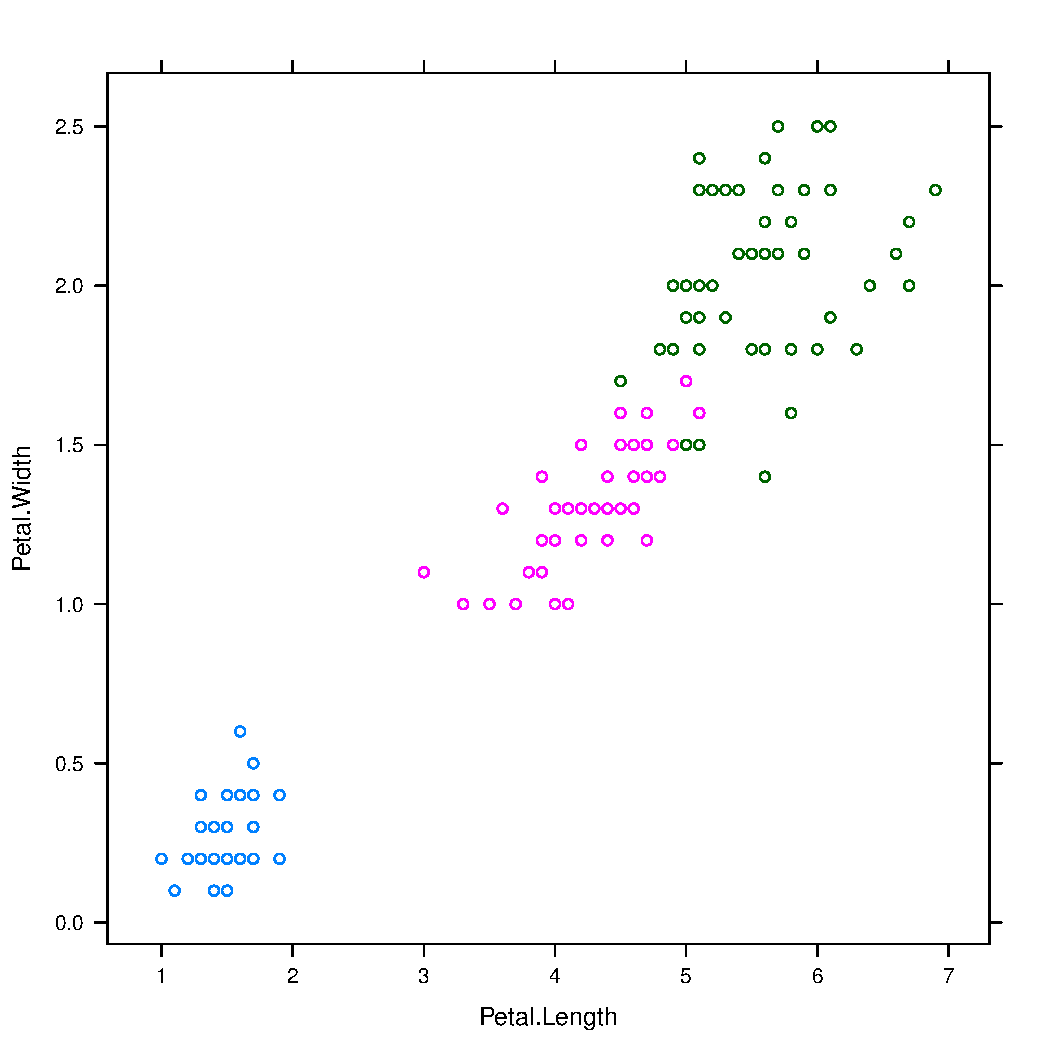
\includegraphics[width=5in, height=4in]{img/xyplot-group.pdf}
    \caption{}
    \label{fig:xyplot-group}
  \end{figure}

\begin{itemize}
\item Scatterplot matrices
\begin{itemize}
\item splom( \~{} cbind(GNP.deflator,GNP,Unemployed,Armed.Forces,Population,Year,Employed),  data = longley)
\item splom( \~{} cbind(pop15,pop75,dpi), data = LifeCycleSavings)
\item splom( \~{} cbind(Murder, Assault, Rape), data = USArrests)
\item splom( \~{} cbind(CONT, INTG, DMNR), data = USJudgeRatings)
\item splom( \~{} cbind(area,peri,shape,perm), data = rock)
\item splom( \~{} cbind(Air.Flow, Water.Temp, Acid.Conc., stack.loss), data = stackloss)
\item splom( \~{} cbind(Fertility,Agriculture,Examination,Education,Catholic,Infant.Mortality), data = swiss)
\item splom(\~{} cbind(Fertility,Agriculture,Examination), data = swiss) (positive and negative)
\end{itemize}
\item Dot charts
\begin{itemize}
\item dotchart(USPersonalExpenditure)
\item dotchart(t(USPersonalExpenditure))
\item dotchart(WorldPhones) (transpose is no good)
\item freeny.x is no good, neither is volcano
\item dotchart(UCBAdmissions\{[\},,1\{]\})
\item dotplot(Survived \~{} Freq | Class, groups = Sex, data = B)
\item dotplot(Admit \~{} Freq | Dept, groups = Gender, data = C)
\end{itemize}
\item Mosaic plot
\begin{itemize}
\item mosaic( \~{} Survived + Class + Age + Sex, data = Titanic) (or just mosaic(Titanic))
\item mosaic( \~{} Admit + Dept + Gender, data = UCBAdmissions)
\end{itemize}
\item Spine plots
\begin{itemize}
\item spineplot(xtabs(Freq \~{} Admit + Gender, data = UCBAdmissions))
\item \# rescaled barplot
\end{itemize}
\item Quantile-quantile plots: There are two ways to do this. One way is to compare two independent samples (of the same size). qqplot(x,y). Another way is to compare the sample quantiles of one variable to the theoretical quantiles of another distribution.
\end{itemize}


Given two samples \(x_{1}\), \(x_{2}\), \ldots{}, \(x_{n}\), and \(y_{1}\), \(y_{2}\), \ldots{}, \(y_{n}\), we may find the order statistics \(x_{(1)}\leq x_{(2)}\leq\cdots\leq x_{(n)}\) and \(y_{(1)}\leq y_{(2)}\leq\cdots\leq y_{(n)}\). Next, plot the \(n\) points \((x_{(1)},y_{(1)})\), \((x_{(2)},y_{(2)})\), \ldots{}, \((x_{(n)},y_{(n)})\).

It is clear that if \(x_{(k)}=y_{(k)}\) for all \(k=1,2,\ldots,n\), then we will have a straight line. It is also clear that in the real world, a straight line is NEVER observed, and instead we have a scatterplot that hopefully had a general linear trend. What do the rules tell us? 

\begin{itemize}
\item If the \(y\)-intercept of the line is greater (less) than zero, then the center of the \(Y\) data is greater (less) than the center of the \(X\) data.
\item If the slope of the line is greater (less) than one, then the spread of the \(Y\) data is greater (less) than the spread of the \(X\) data.
\end{itemize}
\subsection{Lattice Graphics}
\label{sec-1-6-3}

\label{sub:Lattice-Graphics}

The following types of plots are useful when there is one variable of interest and there is a factor in the data set by which the variable is categorized. 

It is sometimes nice to set \texttt{lattice.options(default.theme = "col.whitebg")}


\paragraph*{Side by side boxplots}


\begin{verbatim}
library(lattice)
bwplot(~weight | feed, data = chickwts)
\end{verbatim}





\begin{figure}[ht!]
    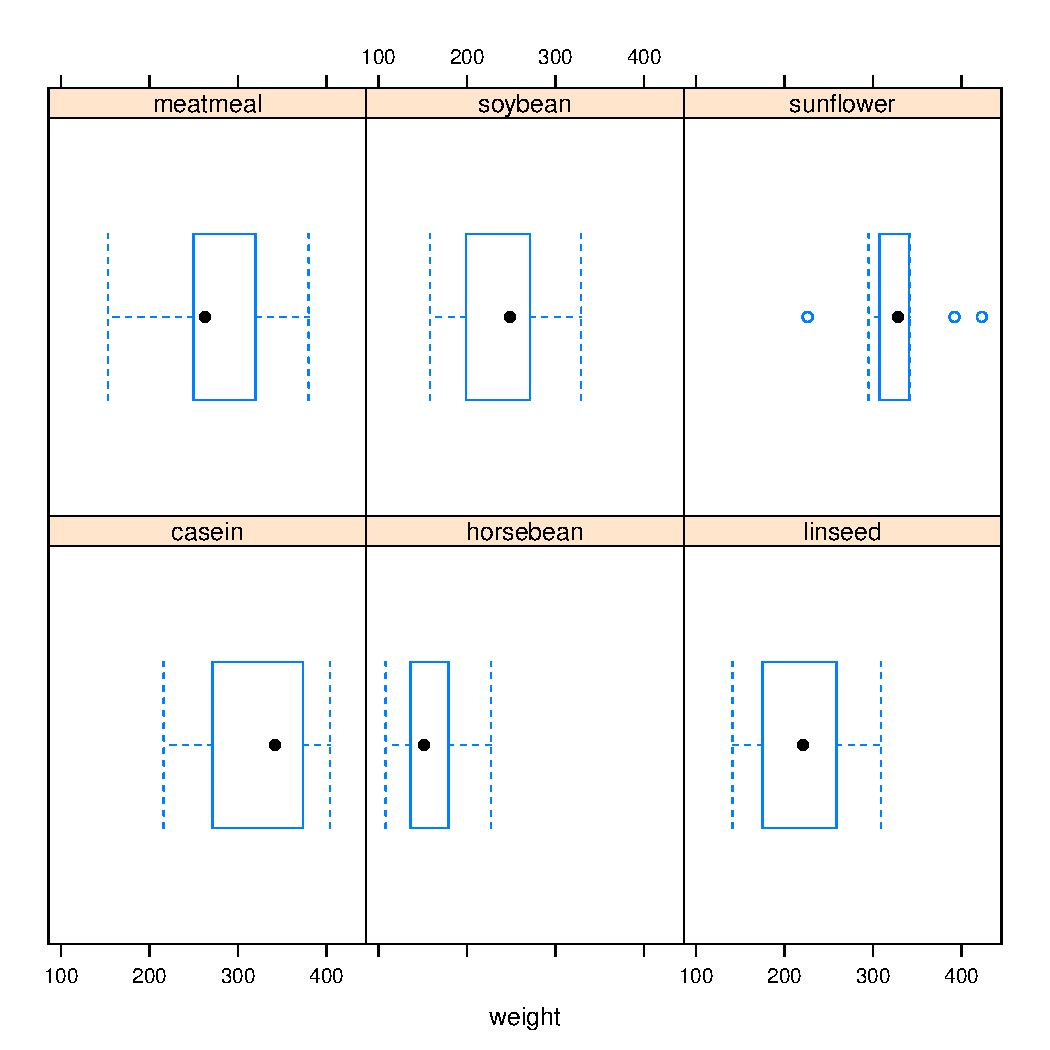
\includegraphics[width=5in, height=4in]{img/bwplot.pdf}
    \caption{Boxplots of \texttt{weight} by \texttt{feed} type in the \texttt{chickwts} data}
    \label{fig:bwplot}
  \end{figure}


\paragraph*{Histograms}


\begin{verbatim}
histogram(~age | education, data = infert)
\end{verbatim}





\begin{figure}[ht!]
    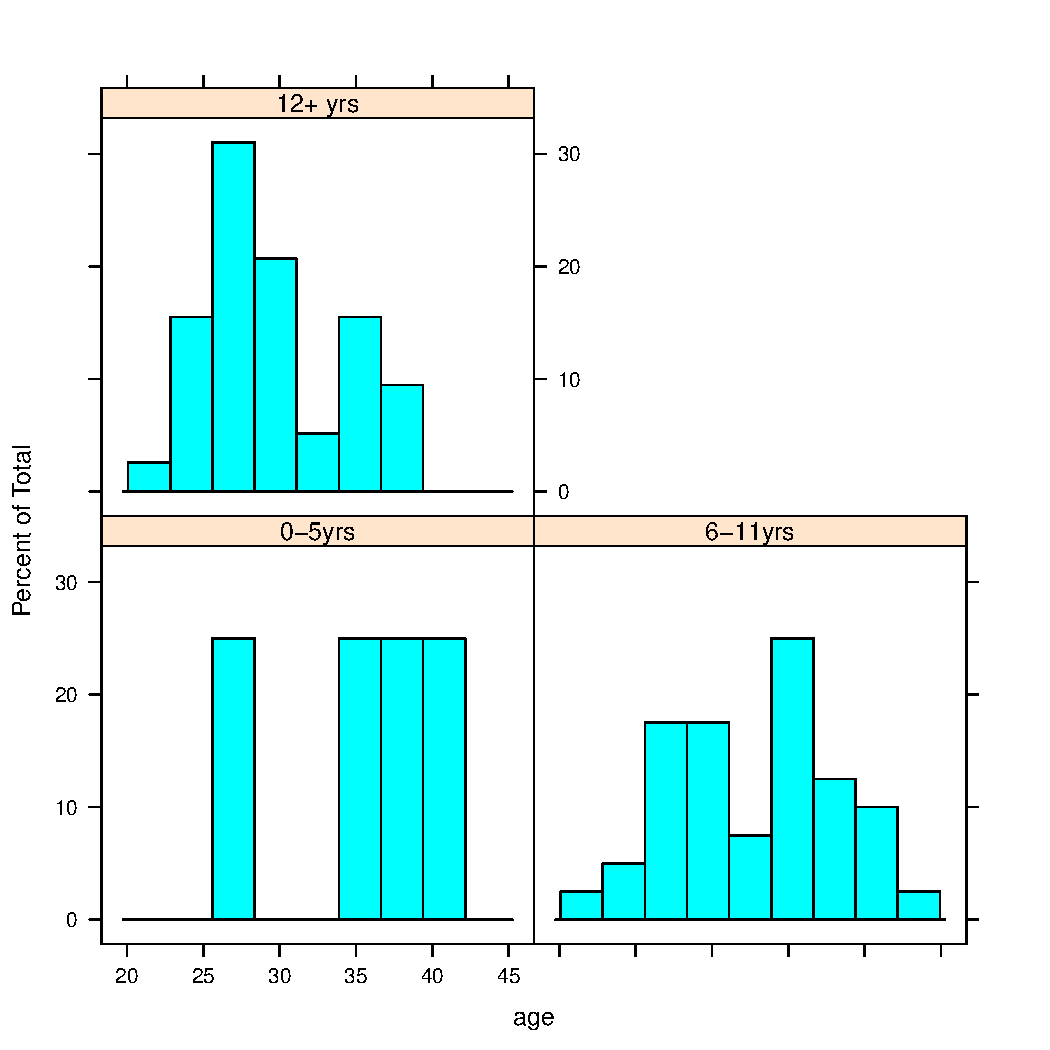
\includegraphics[width=5in, height=4in]{img/histograms-lattice.pdf}
    \caption[Histograms of \texttt{age} by \texttt{education} level]{Histograms of \texttt{age} by \texttt{education} level from the \texttt{infert} data}
    \label{fig:histograms-lattice}
  \end{figure}



\paragraph*{Scatterplots}


\begin{verbatim}
xyplot(Petal.Length ~ Petal.Width | Species, data = iris)
\end{verbatim}





\begin{figure}[ht!]
    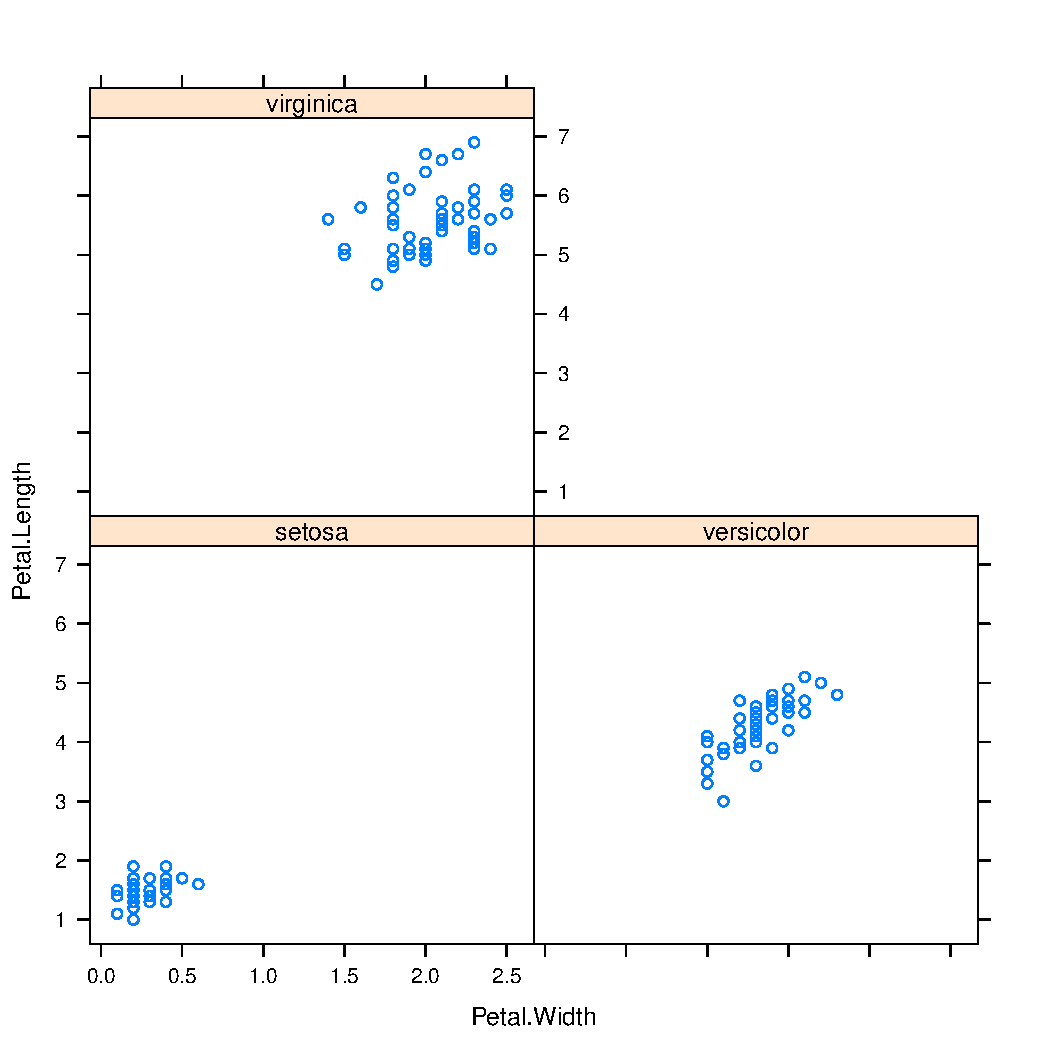
\includegraphics[width=5in, height=4in]{img/xyplot.pdf}
    \caption[An \texttt{xyplot} of \texttt{Petal.Length} versus \texttt{Petal.Width} by \texttt{Species}]{An \texttt{xyplot} of \texttt{Petal.Length} versus \texttt{Petal.Width} by \texttt{Species} in the \texttt{iris} data}
    \label{fig:xyplot}
  \end{figure}


\paragraph*{Coplots}


\begin{verbatim}
coplot(conc ~ uptake | Type * Treatment, data = CO2)
\end{verbatim}





\begin{figure}[ht!]
    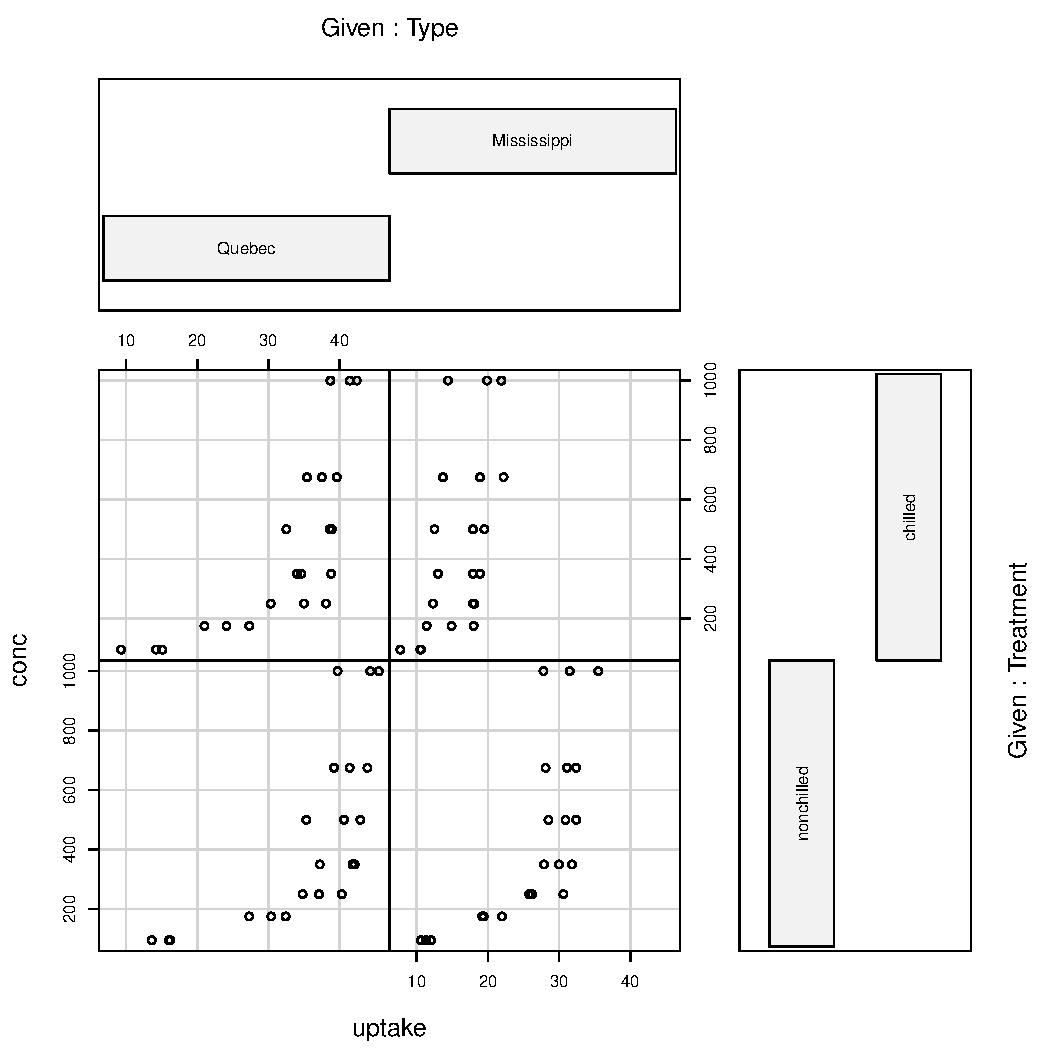
\includegraphics[width=5in, height=4in]{img/coplot.pdf}
    \caption[A \texttt{coplot} of \texttt{conc} versus \texttt{uptake} by \texttt{Type} and \texttt{Treatment}]{A \texttt{coplot} of \texttt{conc} versus \texttt{uptake} by \texttt{Type} and \texttt{Treatment} in the \texttt{CO2} data}
    \label{fig:coplot}
  \end{figure}


\newpage{}
\section*{Chapter Exercises}
\addcontentsline{toc}{section}{Chapter Exercises}
\setcounter{thm}{0}

\paragraph*{Directions: }

Open \textsf{R} and issue the following commands at the command line to get started. Note that you need to have the \texttt{RcmdrPlugin.IPSUR} package installed, and for some exercises you need the \texttt{e1071} package.


\begin{verbatim}
library(RcmdrPlugin.IPSUR)
data(RcmdrTestDrive)
attach(RcmdrTestDrive)
names(RcmdrTestDrive)
\end{verbatim}

To load the data in the \textsf{R} Commander (\texttt{Rcmdr}), click the \textsf{Data Set} button, and select \texttt{RcmdrTestDrive} as the active data set. To learn more about the data set and where it comes from, type \texttt{?RcmdrTestDrive} at the command line.

\begin{xca}
\label{xca:summary-RcmdrTestDrive}

Perform a summary of all variables in \texttt{RcmdrTestDrive}. You can do this with the command \texttt{summary(RcmdrTestDrive)}.

Alternatively, you can do this in the \texttt{Rcmdr} with the sequence \textsf{Statistics} \textsf{\(\triangleright\) Summaries} \textsf{\(\triangleright\) Active Data Set}. Report the values of the summary statistics for each variable.

\end{xca}

\begin{xca}
Make a table of the \texttt{race} variable. Do this with \textsf{Statistics} \textsf{\(\triangleright\) Summaries} \textsf{\(\triangleright\) IPSUR - Frequency Distributions}...

\begin{enumerate}
\item Which ethnicity has the highest frequency?
\item Which ethnicity has the lowest frequency?
\item Include a bar graph of \texttt{race}. Do this with \textsf{Graphs} \textsf{\(\triangleright\)} \textsf{IPSUR - Bar Graph}...
\end{enumerate}

\end{xca}

\begin{xca}
Calculate the average \texttt{salary} by the factor \texttt{gender}. Do this with \textsf{Statistics} \textsf{\(\triangleright\) Summaries} \textsf{\(\triangleright\) Table of Statistics}... 
\begin{enumerate}
\item Which \texttt{gender} has the highest mean \texttt{salary}?
\item Report the highest mean \texttt{salary}.
\item Compare the spreads for the genders by calculating the standard deviation of \texttt{salary} by \texttt{gender}. Which \texttt{gender} has the biggest standard deviation?
\item Make boxplots of \texttt{salary} by \texttt{gender} with the following method:
   \begin{quote}
   On the \texttt{Rcmdr}, click \textsf{Graphs} \textsf{\(\triangleright\)} \textsf{IPSUR - Boxplot}...
   In the \textsf{Variable} box, select \texttt{salary}.
   Click the \textsf{Plot by groups}... box and select \texttt{gender}. Click \textsf{OK}.
   Click \textsf{OK} to graph the boxplot.
   \end{quote}
   How does the boxplot compare to your answers to (1) and (3)?
\end{enumerate}
\end{xca}

\begin{xca}
For this problem we will study the variable \texttt{reduction}.
\begin{enumerate}
\item Find the order statistics and store them in a vector \texttt{x}. \emph{Hint:} \texttt{x <- sort(reduction)}
\item Find \(x_{(137)}\), the 137\(^{\mathrm{th}}\) order statistic.
\item Find the IQR.
\item Find the Five Number Summary (5NS).
\item Use the 5NS to calculate what the width of a boxplot of \texttt{reduction} would be.
\item Compare your answers (3) and (5). Are they the same? If not, are they close?
\item Make a boxplot of \texttt{reduction}, and include the boxplot in your report. You can do this with the \texttt{boxplot} function, or in \texttt{Rcmdr} with \textsf{Graphs} \textsf{\(\triangleright\)} \textsf{IPSUR - Boxplot}...
\item Are there any potential/suspected outliers? If so, list their values. \emph{Hint:} use your answer to (a).
\item Using the rules discussed in the text, classify answers to (8), if any, as \emph{potential} or \emph{suspected} outliers.
\end{enumerate}
\end{xca}

\begin{xca}
In this problem we will compare the variables \texttt{before} and \texttt{after}. Don't forget \texttt{library(e1071)}.
\begin{enumerate}
\item Examine the two measures of center for both variables. Judging from these measures, which variable has a higher center?
\item Which measure of center is more appropriate for \texttt{before}? (You may want to look at a boxplot.) Which measure of center is more appropriate for \texttt{after}?
\item Based on your answer to (2), choose an appropriate measure of spread for each variable, calculate it, and report its value. Which variable has the biggest spread? (Note that you need to make sure that your measures are on the same scale.)
\item Calculate and report the skewness and kurtosis for \texttt{before}. Based on these values, how would you describe the shape of \texttt{before}?
\item Calculate and report the skewness and kurtosis for \texttt{after}. Based on these values, how would you describe the shape of \texttt{after}?
\item Plot histograms of \texttt{before} and \texttt{after} and compare them to your answers to (4) and (5).
\end{enumerate}
\end{xca}

\begin{xca}
Describe the following data sets just as if you were communicating with an alien, but one who has had a statistics class. Mention the salient features (data type, important properties, anything special). Support your answers with the appropriate visual displays and descriptive statistics.
\begin{enumerate}
\item Conversion rates of Euro currencies stored in \texttt{euro}.
\item State abbreviations stored in \texttt{state.abb}.
\end{enumerate}
\end{xca}

\end{document}